% !TEX root = ../thesis.tex
\chapter{基于相似性学习的深度图像抠图方法}
\section{引言}
在前几章中,我们分别研究了数据驱动的相似性学习在无监督的度量学习和半监督的约束聚类中的应用情况,本章将着重研究相似性学习在具有监督信息的自然图像抠图问题中的算法应用。与前几章中不同的是,在本章中我们将着重关注如何通过数据驱动的网络模型学习相似性的生成方式,而不是直接学习相似性的数值。

自然图像抠图(natural image matting)是计算机视觉中的重要任务之一。它在图像或视频编辑、合成和电影后期制作方面具有大量应用\cite{wang2008image,aksoy2017designing,lutz2018alphagan,xu2017deep,samplenet}。抠图问题已引起学术界的极大兴趣,并且在过去十年中被广泛地研究。
自然图像抠图是将前景对象与背景图相分离的问题并估计它们之间的过渡取值的问题。数字图像抠图将输入的自然图像视为前景图和背景图的合成图像,旨在估计前景图像的不透明度。其预测结果是alpha半透明遮罩(alpha matte),表示每个像素在前景和背景之间的过渡取值\cite{wang2008image}。

在数学形式上,观察到的RGB图像$ I $被建模为前景图像$ F $和背景图像$ B $的凸组合的形式\cite{chuang2001bayesian,wang2008image}:
\begin{equation}
I_p = \alpha_pF_p + (1-\alpha_p)B_p, \quad \alpha_p \in [0,1],
\label{eq5:matting}
\end{equation}
其中$ \alpha_p $表示要在像素位置$ p $所估计的alpha遮罩值。如果$ \alpha_p $的取值不是$0$或者$1$,则在像素位置$p$的图像像素值即是由前景和背景混合而成。由于前景颜色$ F_p $、背景颜色$ B_p $和alpha取值$ \alpha_p $都是未知的,所以图像抠图的原始数学定义是一个欠定问题。因此,大多数先前的传统抠图算法都会在抠图问题中引入一个比较强的归纳偏置(inductive bias)。同时,在大多数抠图任务中,都将trimap图像作为粗略标注提供给算法,trimap图像上标注有已知的前景和背景区域以及需要预测的未知区域。

在基于相似性和基于采样的算法中广泛采用的基本思想之一是从具有相似外观的图像区域中借用信息。通常,传统的基于相似性的方法\cite{levin2008closed,he2010fast,chen2013knn,aksoy2017designing}通过参考输入图像中不同区块间的外观相似性,将不透明度或透明度在像素之间进行传播,以生成alpha遮罩值。基于采样的算法\cite{wang2007optimized,gastal2010shared,he2011global,feng2016cluster}一般从前景和背景中借用一对采样区块,以基于某些特定假设来估计未知区域中每个像素的alpha值。
先前基于相似性和基于采样的方法的一个不足点是,它们无法处理trimap中仅存在背景区域和未知区域标注的情况。这是因为这些方法必须同时利用前景和背景信息来估计alpha取值,在没有前景标注的情况下,这些算法无法正常计算。

受益于Adobe Image Matting数据集\cite{xu2017deep},近年来出现了更多基于学习的图像抠图方法 \cite{xu2017deep,lutz2018alphagan,lu2019indices,samplenet,cai2019disentangled,hou2019context}。大多数基于学习的方法都使用神经网络先验作为归纳偏置并直接预测Alpha遮罩值。

部分基于深度学习的抠图方法\cite{samplenet,cai2019disentangled}更是潜在地利用了相似外观的图像区域具有相似alpha遮罩值这一假设作为归纳偏置,从而改进了其抠图效果。
SampleNet\cite{samplenet}通过其方法中采用的图像补全(image inpainting)网络\cite{yu2018generative}实现传播,以进行前景和背景估计,再通过采样方法预测alpha值,而不是通过传播不透明度直接进行预测。此外,图像补全网络中的传播行为仅作用在具有强语义的少部分特征上,而不是在高分辨率特征上进行。在AdaMatting\cite{cai2019disentangled}中,作者将卷积长短时记忆(Convolutional LSTM,ConvLSTM)网络\cite{xingjian2015convolutional}引入了它们的网络中,作为网络最后的传播阶段。其中,信息传播是基于ConvLSTM中的卷积和记忆存储部分实现的。
ConvLSTM和直接传播之间并不能看作是等价的计算模块,两者的区别可以类比于LSTM\cite{hochreiter1997long}和Transformer\cite{vaswani2017attention}之间的区别。

本章将先后提出两种基于相似性的深度抠图方法,所提出方法通过数据驱动的监督训练学习基于图像外观信息的像素相似性生成方式,以实现不透明度的信息传播。近几年信息传播在神经网络框架中被广泛地采纳,从自然语言处理\cite{vaswani2017attention,yang2019xlnet}、数据挖掘\cite{kipf2016semi,velivckovic2017graph}到计算机视觉\cite{yu2018generative,wang2018non}都有大量工作通过信息传播的方式改进算法性能。在本章中,我们首先将提出基本的引导上下文注意力抠图(Guided Contextual Attention Matting,GCA Matting)模型,以在深度神经网络中实现基本的信息传播功能。然后在此基础上提出了一种新颖的层次化不透明度传播抠图(Hierarchical Opacity Propagation Matting,HOP Matting)方法,其中,不透明度信息可以在不同语义级别的特征间进行传播。HOP Matting模型中所提出的结构主要由全局HOP模块和局部HOP模块两种传播模块构成。HOP模块基于所提出的引导上下文注意力(Guided Contextual Attention,GCA)机制实现,该机制可以在全卷积神经网络中模拟基于相似性的传统抠图算法的传播过程。在GCA机制中,低级语义特征被用来作为传播过程的引导信息,根据引导信息,该机制对alpha特征进行传播。已知区块和未知区块中的信息被传播到未知区域中具有相似外观的特征区块中。

本章中所提出的图像抠图方法可以从两个不同的角度进行解释。 一方面,可以将引导上下文注意力机制解释为一种具有神经网络先验的基于相似性进行alpha值传播的抠图方法。在低级图像特征间相似度的引导下,未知区域中的区块相互之间对具有高级语义的alpha特征进行共享。
另一方面,所提出的方法也可以看作是引导性的图像补全任务。在这个角度下,根据输入图像的引导,图像抠图任务可以被视为是在alpha遮罩图像上的补全任务。未知区域类比于要在图像补全中待填充的孔洞部分。与通常情况下,从同一图像的背景借用像素的补全方法不同的是,图像抠图在原始RGB图像的引导下在alpha遮罩图像中的已知区域借像素值$ 0 $或$ 1 $来填充未知区域。

\section{相关工作}
大多数自然图像抠图方法可以粗略分为基于相似性的方法\cite{levin2008closed,he2010fast,lee2011nonlocal,chen2013knn,aksoy2017designing},基于采样的方法\cite{wang2007optimized,gastal2010shared,he2011global,feng2016cluster}和基于学习的方法\cite{xu2017deep,lutz2018alphagan,lu2019indices,samplenet,hou2019context,cai2019disentangled}三类。在本节中,我们将回顾一些与该章节相关度较高的基于深度学习的抠图算法。

一般基于深度学习的方法利用深度神经网络通过给定图像和trimap图直接预测alpha遮罩值。
Cho等人\cite{cho2019deep}最先在抠图任务中使用了端到端卷积神经网络(Convolutional Neural Network,CNN),该网络从Closed-form Matting\cite{levin2008closed}和KNN Matting\cite{chen2013knn}中获取alpha值以及归一化的RGB图像作为输入,以更好地利用局部和非局部(nonlocal)结构信息对不同算法生成的alpha值进行融合。
文献\parencite{xu2017deep}中提出了Deep Matting方法作为一个两阶段网络来预测alpha遮罩。在第一阶段中,算法向深层卷积编码器-解码器网络输入图像和相应的trimap,得到粗略预测结果。在第二阶段,通过浅层网络对粗略预测的alpha值进行细化。
Lutz等人\cite{lutz2018alphagan}将生成对抗网络(Generative Adversarial Networks,GAN)引入了图像抠图问题,并使用膨胀卷积来捕获全局上下文信息。
Tang等人\cite{tang2019very}提出了一个名为VDRN的神经网络,该网络包含一个深度残差(residual)编码器和一个复杂的解码器。
AdaMatting\cite{cai2019disentangled}方法将抠图问题分为两个任务,trimap自适应和alpha估计,并使用具有两个不同解码器分支的CNN模型以多任务学习方式处理。
IndexNet Matting\cite{lu2019indices}方法将池化(pooling)操作中的索引作为特征图的函数,并提出了一种通过索引引导的编码器-解码器网络,该网络通过由学习得到的索引信息进行的索引池化和上采样。
Hou和Liu\cite{hou2019context}提出了一个上下文感知(context-aware)网络来预测前景和alpha遮罩值。Context-aware Matting使用两种编码器,一种用于局部特征,另一种用于上下文信息。 

一些方法表明,不对alpha进行直接预测,而更改问题的自由度可以改善网络的性能。
Tang等人\cite{samplenet}提出了SampleNet来逐步地估计前景、背景和alpha遮罩,而不是同时对其进行预测。
Zhang等人\cite{Zhang2019ALF}使用两个解码器分支分别估计前景和背景,然后使用融合分支获得最终预测结果。



\section{深度图像抠图基线网络}
我们所提出的模型使用带有GCA机制的HOP模块以及一个自定义的U-Net\cite{ronneberger2015u}架构实现深度自然图像抠图。在本节中,我们将首先对自定义的U-Net基线网络进行介绍。

\begin{figure}[t]
	\centering
	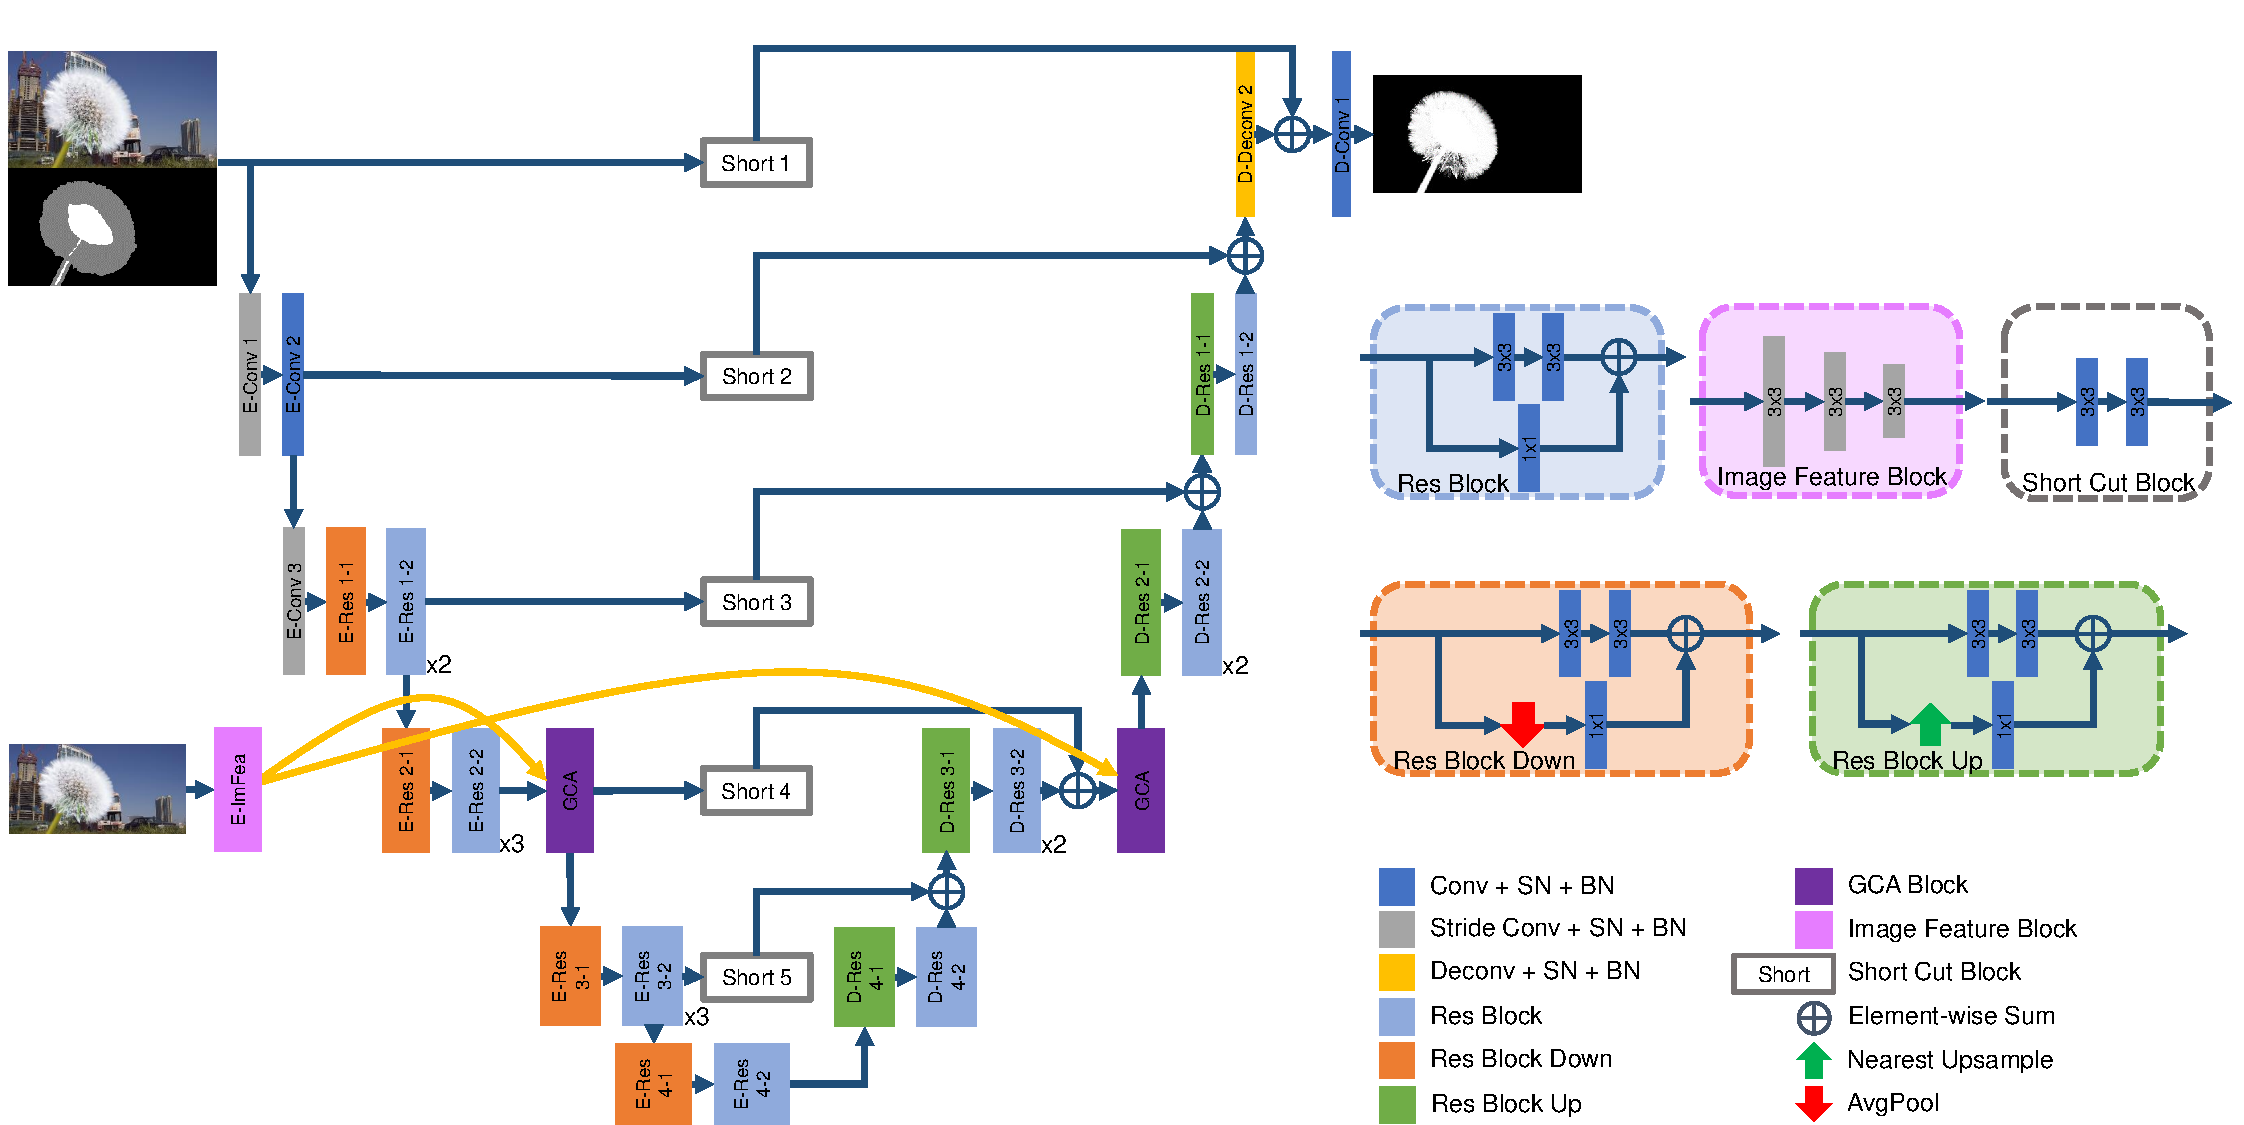
\includegraphics[width = 1\textwidth]{chap5/10261arch1.pdf}
	\bicaption{所提出的GCA Matting的网络结构细节图。基线网络模型具有相同的网络结构,但不具备图中的GCA机制部分以及图像特征模块。原始图像和trimap图像为alpha特征的输入数据,而图像特征模块仅将原始的合成图像作为输入数据。蓝色箭头表示alpha特征流,黄色箭头表示低级语义的图像特征流。GCA:引导上下文注意力;SN:谱归一化;BN:批归一化; $ \times N $:重复$ N $次}{Overview of our proposed guided contextual attention matting framework. The baseline model shares the same architecture without GCA mechanism and image feature block. Original image and trimap are the inputs of alpha feature. Image feature block only takes the original merged image as input. The blue arrows denote alpha feature flow and yellow arrows denote low-level image feature flow. GCA: guided contextual attention; SN: spectral normalization; BN: batch normalization; $ \times N $: replicate $ N $ times}
	\label{fig5:arch}
\end{figure}

\subsection{基线网络结构}
在近几年的图像抠图\cite{lutz2018alphagan,samplenet,lu2019indices}、图像分割\cite{long2015fully}、图像转换\cite{isola2017image}和图像补全\cite{liu2018image}任务中,类U-Net网络结构非常流行。在图\ref{fig5:arch}中给出了具有附带的GCA机制的基线网络结构。图中的网络结构与我们所设计的基线网络模型的唯一区别在于基线网络中没有GCA机制,因此也就没有其上游的图像特征模块(Image Feature Block)。

该基线网络的输入为裁剪后的图像块和3通道独热编码(one-hot encoding)的trimap图,它们被拼接为一个6通道输入。输出是相应的预测alpha遮罩值。
基线网络结构被设计为具有堆叠残差模块(stacked residual blocks)\cite{he2016deep}的编码器-解码器网络。

由于低级图像特征能对在alpha遮罩中保留纹理信息起到至关重要的作用,因此在我们自定义的基线模型中,解码器在上采样块之前(而不是在每个上采样块之后)对编码器输出的特征进行合并。这是因为预期中这些编码器特征具有更多的低级图像特征,而这样的设计可以避免在低级特征上进行更多的卷积计算。我们还使用了具有两层卷积层的跳层(short cut)块来对齐编码器特征的通道以进行特征融合。同时,与仅结合了不同的中级特征的典型U-Net结构不同,我们将原始输入直接通过跳层块传递到最后的卷积层。这些特征不与主干网络共享任何计算。因此,此跳层分支仅关注细节上的的纹理和梯度信息。

除了广泛使用的批归一化\cite{ioffe2015batch},我们还将谱归一化\cite{miyato2018spectral}引入每个卷积层,以对网络的Lipschitz常数添加约束达到稳定训练的效果,该设计方案普遍存在于图像生成任务中\cite{brock2018large,zhang2018self}。

\subsection{损失函数}
在所提出的神经网络的训练中,我们仅使用了一个alpha预测损失。alpha预测损失可以定义为每个像素的alpha预测值和标注的真实值之间的绝对差在整个未知区域上的平均值:
\begin{equation}
\mathcal{L} = \frac{1}{|\mathcal{U}|} \sum_{i\in \mathcal{U}}|\hat{\alpha_i}-\alpha_i|,
\label{eq5:loss}
\end{equation}
其中$ \mathcal {U} $表示在trimap中标记为未知区域的像素集合,$ \hat{\alpha_i} $和$ \alpha_i $分别表示像素位置$ i $的alpha遮罩预测值和真实值。

在先前的部分相关工作中,针对深度图像抠图任务,有一些新的损失函数被提出来,例如合成损失函数\cite{xu2017deep},梯度损失函数\cite{samplenet}和Gabor损失函数\cite{li2019inductive}。
Deep Matting\cite{xu2017deep}中使用的合成损失函数是通过计算由真实前景,背景和预测alpha遮罩所合成的预测图像与原始输入图像之间的绝对差作为损失。
梯度损失计算未知区域中alpha预测值梯度和真实值梯度之间的平均绝对差。
文献\parencite{li2019inductive}中提出的Gabor损失通过用一系列Gabor过滤器代替了梯度损失中的梯度算子,旨在能在纹理和梯度方面提供比梯度损失更全面的监督。

我们对这些损失进行了深入的研究,以揭示添加这些不同的损失是否可以使基线模型中的alpha值预测效果得到提升。我们在表\ref{tab5:ablation}中提供了在Composition-1k测试集\cite{xu2017deep}上进行的消融实验结果。如表\ref{tab5:ablation}所示,对预测结果的均方误差(Mean Square Error,MSE)和梯度误差(Gradient error,Grad)评测误差而言,引入合成损失函数不会带来任何显着差异,并且当我们将梯度损失加入到alpha预测损失时,给出的两种评测误差都会增加。尽管采用Gabor损失可以在一定程度上降低Grad梯度误差,但也会稍微提高MSE结果。因此,我们仅在模型中选择alpha预测损失作为唯一的损失函数。


\begin{table}[t]
	\bicaption{基线网络结构上的数据增广和不同损失函数的消融实验结果。定量实验结果测试于Composition-1k测试集。Aug:数据增广;Rec:alpha预测损失;Comp:合成损失;GradL:梯度损失;Gabor:Gabor损失}{Ablation study on data augmentation and different loss functions with baseline structure. The quantitative results are tested on Composition-1k testing set. Aug: data augmentation; Rec: alpha prediction loss; Comp: compositional loss; GradL: gradient loss; Gabor: Gabor loss.}
	\centering
	\setlength{\tabcolsep}{8pt}
	\begin{tabular}{ccccc|cc}  
		\toprule
		Aug&Rec&Comp&GradL&Gabor& MSE & Grad\\% & SAD &Conn
		\midrule
		\checkmark&\checkmark&&& & 0.0106 & 21.53 \\  % & {40.62}& 38.43
		\checkmark&\checkmark&\checkmark&&& 0.0107  & 21.85\\% & 40.85  & 38.73
		\checkmark&\checkmark&&\checkmark& & 0.0108 & 22.51\\ % & 43.62  & 42.19
		\checkmark&\checkmark&&&\checkmark & 0.0109 & 20.66\\ % & 42.53  & 40.84   
		&\checkmark&&& & 0.0146 & 32.01 \\%& 51.15& 51.52
		\bottomrule
	\end{tabular}
	\label{tab5:ablation}
\end{table}

\subsection{数据增广方法}
\label{sec5:aug}

由于文献\parencite{xu2017deep}中所提出的目前最主要的图像抠图数据集仅包含431个用于训练的前景对象,所以我们将数据增广视为基线模型的必须部分。
本节中我们将对一系列模型训练中使用的数据增广方案进行介绍。

首先,延续文献\parencite{samplenet}中的数据增广方案,我们以0.5的概率在前景图集合中随机选择两个前景物体图像,并将它们叠加组合以获得一个新的前景对象以及一个新的alpha图像作为采样数据。随后,以0.25的概率前景对象和alpha图像的大小将被调整为$640 \times 640 $,这样网络模型几乎可以看到整个前景图像,而不是裁剪后的局部图像块。然后,在前景图像和相应的alpha图像上进行随机的仿射变换。在此仿射变换中,我们定义了随机旋转,缩放,斜切以及垂直和水平翻转。再后,通过5到29中采样随机数作为像素数对alpha图像进行膨胀和腐蚀来生成trimap。获得trimap后,我们分别随机从每个前景图像中、alpha图和trimap图中的对应位置裁剪一个$ 512 \times 512 $的区块,所有裁剪的区块的中心像素都落在trimap图的未知区域上。然后将前景图像转换到HSV空间,并对色度,饱和度和明度分别施加不同的噪声。
最后,我们从MS COCO数据集\cite{lin2014microsoft}中为每个增广后的前景块随机选择一个背景图像,并将其合成为一张图像作为原始输入图像。

为了证明数据增广的有效性,我们进行了一个只包含最少数据增广的实验。在这种情况下,仅保留两个必要的操作,即图像裁剪和trimap图的膨胀生成。此实验中不包括更多的例如随机图像缩放和翻转这些在大多数先前的深度图像抠图方法\cite{xu2017deep,lutz2018alphagan,samplenet,lu2019indices}中被广泛使用的增广方式。我们将此实验设置视为无数据增广。实验结果被列在表\ref{tab5:ablation}中。我们可以看到,在不进行额外数据增广的情况下,我们的基线模型已经可以与Deep Matting方法的效果相媲美。

\section{引导上下文注意力抠图模型}
本节将对所提出的仅包含单层次引导上下文注意力机制的GCA Matting模型进行介绍。完整的引导上下文注意力机制包含两种组件,一个是用于低级图像特征抽取的图像特征提取器,另一个是用于信息传播的引导上下文注意力模块。

\begin{figure}[t]
	\centering
	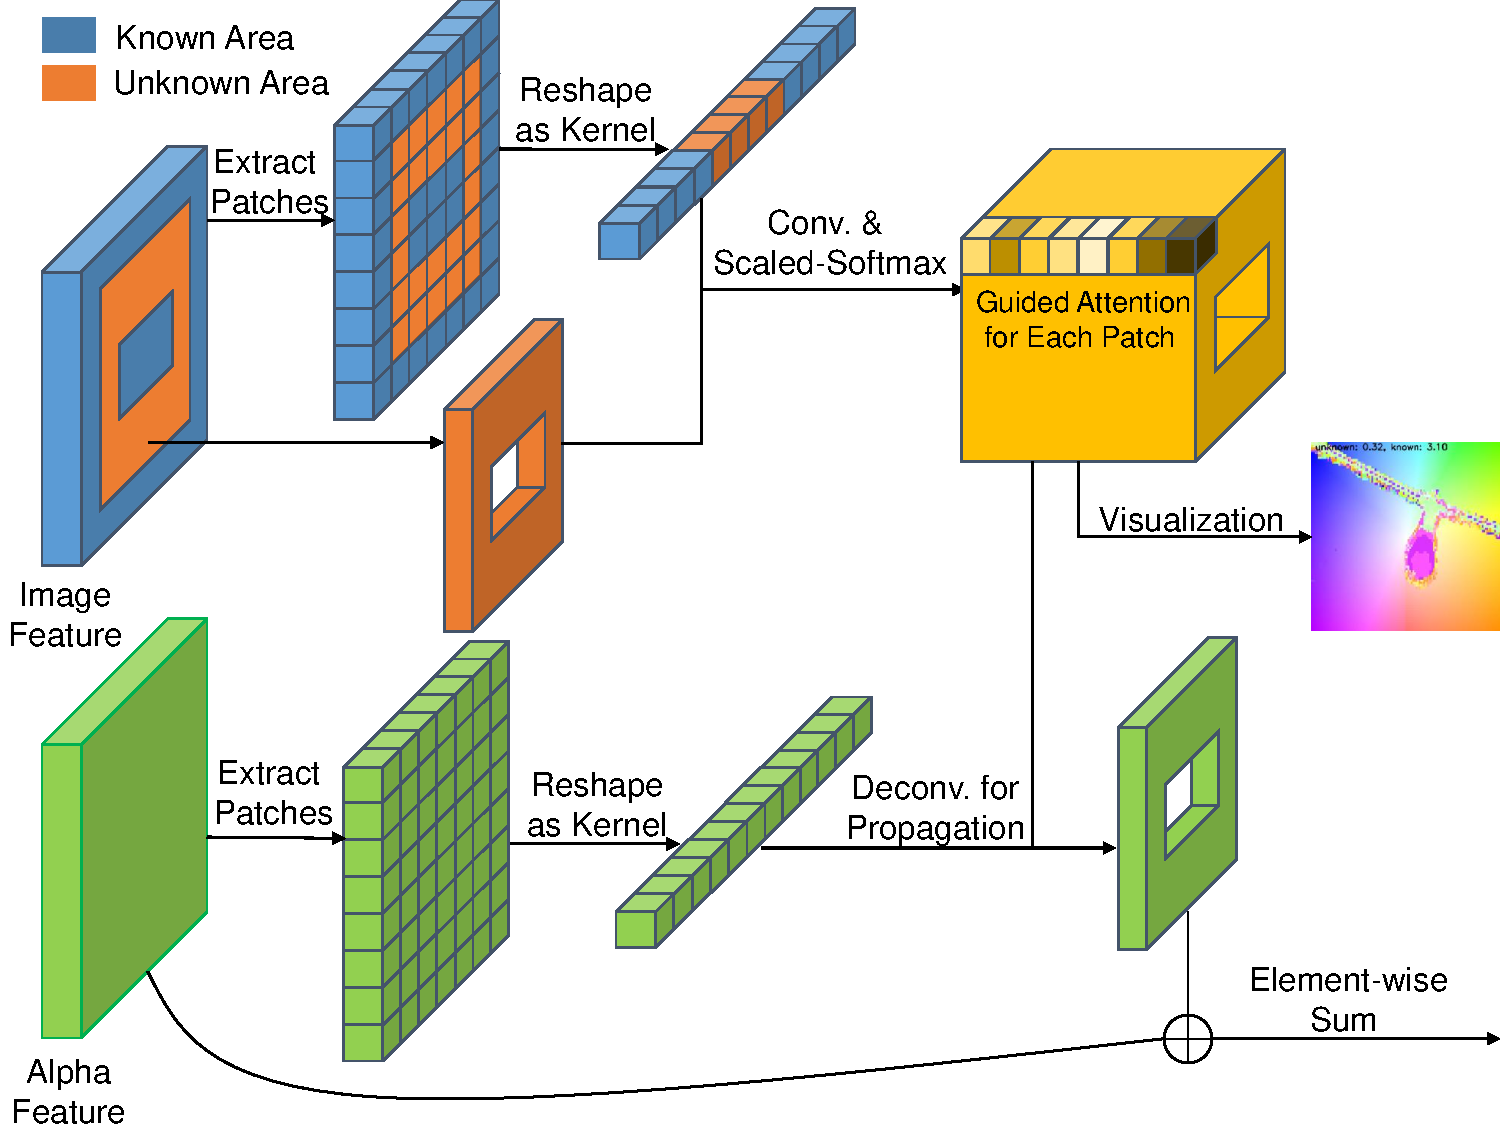
\includegraphics[width = 0.85\columnwidth]{chap5/10261block.pdf}
	\bicaption{引导上下文注意力模块图示。计算过程通过卷积或转置卷积进行实现。为了保持图示整洁,该图中未显示另外两个用于特征对齐的$1\times 1$的卷积层。一个在提取区块之前应用于输入的图像特征,另一个在逐元素求和之前应用于传播结果}{The illustration of the guided contextual attention block. Computation is implemented as a convolution or a deconvolution. Two additional $ 1\times 1 $ convolutional layers for adaptation are not shown in this figure to keep neat. One is applied to the input image feature before extracting patches, and the other one is applied to the result of propagation before the element-wise summation}
	\label{fig5:gca}
\end{figure}

\subsection{低级图像特征}

大多数基于相似性的方法都具有一个基本的归纳偏置,即外观几乎相同的局部区块应具有相似的不透明度。该归纳偏置允许基于相似性的抠图算法将alpha值从trimap图中的已知区域传播到未知区域,这通常可以产生非常出色的alpha预测效果。

因此,我们在所提出的框架中定义了两个不同的特征流(图\ref{fig5:arch}):alpha特征流(蓝色箭头)和图像特征流(黄色箭头)。其中alpha特征是从由原始图像和trimap图拼接产生的6通道输入生成的。最终的alpha遮罩值可以直接从该特征中预测,故称为alpha特征。低级图像特性与高级alpha特征形成对比,这些特征仅由具有步长(stride)为2的三个卷积层序列从输入图像生成,这类似于传统的基于相似性的方法中所用到的的局部颜色统计量。

具体来说,alpha特征包含不透明度信息,而低级图像特征包含外观信息。
在提供不透明度和外观信息的情况下,GCA机制可以学习到一个前几章中所多次用到的相似性图,并通过类似于基于相似性的抠图方法进行不透明度传播。
换句话说,我们利用低级图像特征来指导alpha特征上的信息流动。

\subsection{引导上下文注意力模块}
受文献\parencite{yu2018generative}中上下文注意力模块的启发,我们在抠图问题中引入了引导上下文注意力模块。

如图\ref{fig5:gca}所示,引导上下文注意力同时利用了图像特征和alpha特征。首先图像特征被分为已知部分和未知部分,并从全部的图像特征中抽取$3\times 3$的区块。每个特征块表示一个特定未知的外观信息。我们将特征块变形为卷积核。为了能够对一个中心$ (x,y)$在未知区域的图像特征块$ U_{x,y} $和一个中心在$ (x',y') $的图像特征块$ I_{x', y'} $之间的相关性进行度量,相似性被定义为归一化的内积形式:
\begin{equation}
	s_{(x,y), (x',y')} = 	
	\begin{cases}
	\lambda \quad &(x,y)=(x',y');\\
	\langle \frac{U_{x, y}}{\|U_{x, y}\|},\frac{I_{x', y'}}{\|I_{x', y'}\|}\rangle \quad &\mathrm{otherwise},	
	\end{cases}
\end{equation}
其中$ U_{x, y}\in\mathcal{U}$也是图像特征块集合 $ \mathcal{I} $中的一个元素,即$ \mathcal{U} \subseteq \mathcal{I} $。常数$ \lambda $ 为惩罚参数,可以避免未知区域的特征块和自身之间产生很大的相关性,在模型中我们采用$ \lambda =-10^4$。在实现中,该相关性可以通过未知区域特征块与图像特征块经由变形生成的卷积核进行卷积计算得到。给定一个相关性,则可以在$ (x',y') $维度上进行归一化指数函数(softmax)计算,得到每个特征区块上的引导注意力值:
\begin{equation}
	a_{(x,y), (x',y')} = \mathrm{softmax}(w(\mathcal{U}, \mathcal{K}, x',y')s_{(x,y), (x',y')}),
\end{equation}
\begin{equation}
w(\mathcal{U}, \mathcal{K}, x',y') = \begin{cases}
\mathrm{clamp}(\sqrt{\frac{|\mathcal{U}|}{|\mathcal{K}|}}) \quad I_{x',y'} \in \mathcal{U};\\
\mathrm{clamp}(\sqrt{\frac{|\mathcal{K}|}{|\mathcal{U}|}}) \quad I_{x',y'} \in \mathcal{K},
\end{cases}
\label{eq5:weight}
\end{equation}
\begin{equation}
\mathrm{clamp}(\phi) = \mathrm{min}(\mathrm{max}(\phi, 0.1), 10),
\end{equation}
其中$ w(\cdot)$是权重函数,$ \mathcal{K} = \mathcal{I}-\mathcal{U} $是来自已知区域的图像特征块集合。与图像补全任务不同的是,trimap图中未知区域的面积不受任何控制。在许多输入的trimap图中,存在极大的未知区域而几乎没有已知的像素。因此,仅将不透明度信息从已知区域传播到未知部分通常是不可行的。在所提出的引导上下文注意力机制中,我们让未知部分同时借用已知区域和未知区域中的特征。根据每个区域的面积,通过公式(\ref{eq5:weight})中所定义的权重函数,将不同的权重分配给已知和未知的区域。如果已知区域的面积较大,则已知区域的特征块可以传达更准确的外观信息,从而暴露出前景和背景之间的差异,因此,我们将给已知区域特征块分配较大的权重。而如果未知区域的面积很大,则已知区域的图像特征块只会提供一些局部的外观信息,这可能会损害到不透明度的传播,所以,我们将较小的权重分配给已知区域特征块。

当从图像特征得到引导注意力值后,可以根据由引导注意力值所定义的相似性矩阵,在alpha特征上进行信息传播。
与图像特征类似,从alpha特征中提取特征块并将其变形为卷积核。信息传播过程可以通过引导注意力值与变形后的alpha特征块之间的转置卷积计算完成。该转置卷积可在未知区域中重建alpha特征,并对转置卷积中相互覆盖的像素值取平均。最后,我们通过逐元素求和对输入的alpha特征和传播结果进行融合。这种逐元素求和作为一个残差连接可以对模型训练起到稳定作用。

在此方法所隐含的相似性图中,每个节点都有两种不同的特征,即不透明度alpha特征和图像外观特征。图像外观特征仅用于生成相似性图中的边缘权重,而不透明度alpha特征是实际上的待传播信息。从图\ref{fig5:gca_comp}可以从图的角度看出所提出的GCA模块与上下文注意力机制及自注意力机制之间的区别。GCA机制中每个点对应于两个不同空间的特征,一个用于引导,一个用于承载信息。可以看出在不同的特征空间上数据点之间的相似性是不相同的,这可以类比于前文多模态约束传播中不同模态上的相似性矩阵的不同。

\begin{figure}[t]
	\centering
	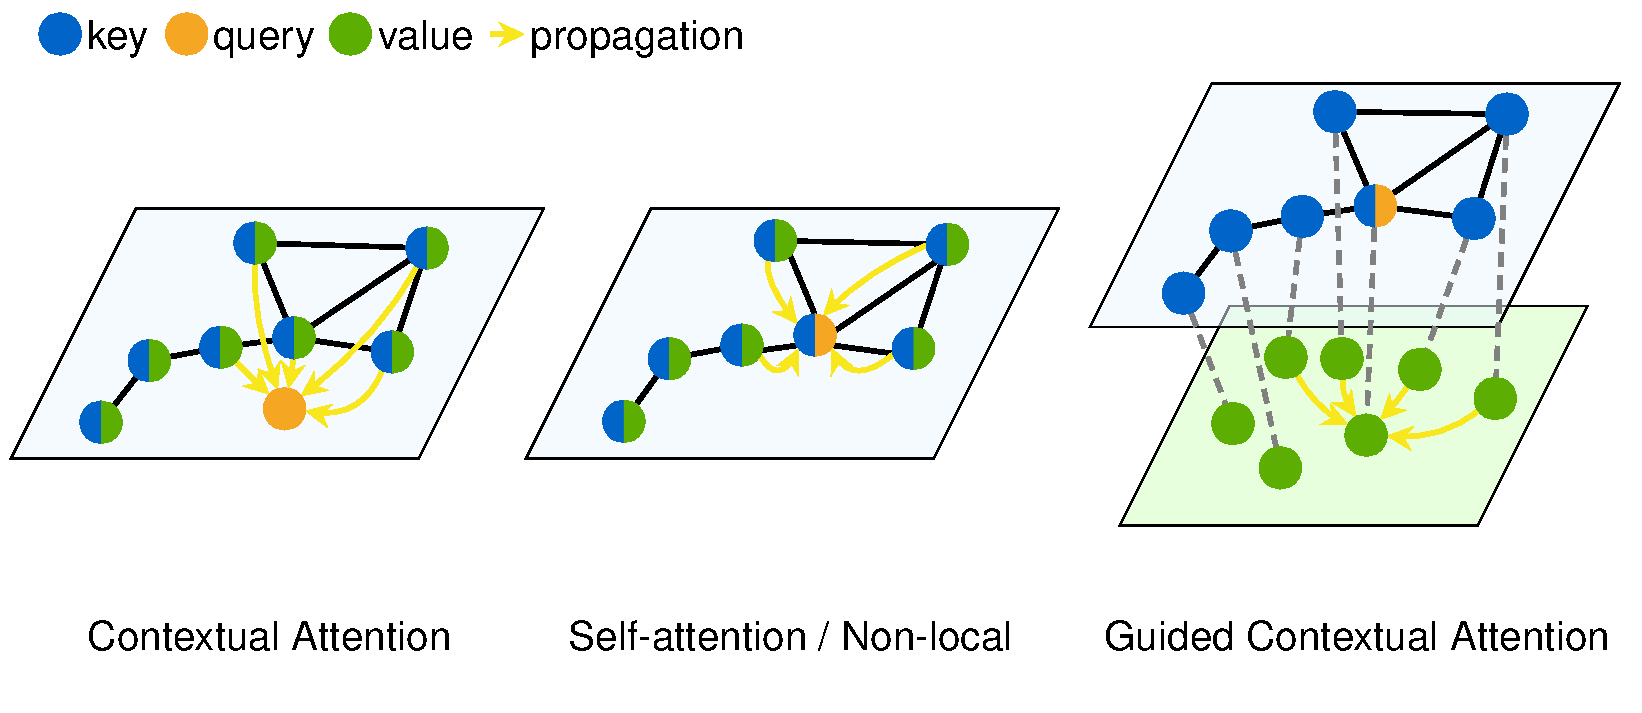
\includegraphics[width = 0.85\columnwidth]{chap5/GCA-compare.pdf}
	\bicaption{在相似性图角度下上下文注意力、自注意力/Non-local和引导上下文注意力的对比。每个平面代表一种特征空间}{Comparison between Contextual Attention, Self-Attention/Non-local and Guided Contextual Attention through the lens of affinity graph. Each plain indicate a feature space }
	\label{fig5:gca_comp}
\end{figure}

\subsection{神经网络实现细节}
多数基于相似性的经典抠图方法最终产生一个依赖于图拉普拉斯的闭式解\cite{levin2008closed,lee2011nonlocal,chen2013knn}。闭式解可以被看作是信息传播算子的不动点,或者是传播迭代趋于无穷时收敛到的极限值\cite{zhou2004learning}。
在基于相似性抠图的经典算法中,图拉普拉斯矩阵大多通过手工设计的固定计算方式生成,而不依赖于数据本身的分布特性。在本章所提出的两个抠图模型中,所使用到的相似性矩阵皆是通过神经网络特征计算得出,然而,神经网络参数本身是通过训练数据学习而来。所以,本章所提出的抠图方法本质上是通过数据驱动,在训练集上学习相似性矩阵的生成方式,以此提升纯端到端的深度抠图网络的性能。同时,不同的图像外观特征分支也会生成不同的相似性矩阵。因此,我们在主干网络中对称地将两个引导上下文注意力模块插入到同一层次的编码器和解码器上。该设计目的在于使数据在模型中进行更多次的传播,并充分利用不透明度的信息流。

当在更高分辨率特征上计算引导上下文注意力时,模型就可以关注到更细节的外观信息。但是,另一方面,注意力模块的计算复杂度为$ O(c(hw)^2)$,其中$ c、h、w $分别是特征图的通道、高度和宽度。因此,我们将两个引导注意力模块添加到尺寸层次为$ 64 \times 64 $的网络阶段中。

在Adobe Image Matting数据集\cite{xu2017deep}上,我们对GCA Matting的网络进行了$ 200,000 $次迭代训练,批大小(batch size)为40。训练中使用了$ \beta_1 = 0.5 $和$ \beta_2 = 0.999 $的Adam优化器\cite{kingma2014adam}执行优化。学习率初始化为$ 4 \times 10^{-4} $,在学习率上使用了预热(warmup)和余弦衰减(cosine decay)\cite{loshchilov2016sgdr,goyal2017accurate,he2019bag}策略。

\section{层次化不透明度传播抠图模型}
在上一节所提出的GCA Matting模型的基础上,为了在高分辨率级别的特征上对整个输入图像实现直接的不透明度信息传播,本节提出了新的层次化不透明度传播(Hierarchical Opacity Propagation,HOP)结构,其中所提出的神经网络结构可以看作是每层具有不同的图连接权重的多层图卷积网络\cite{kipf2016semi},且不透明度可以在任意两个像素之间实现传播。
在本节中,我们将首先介绍层次化不透明度传播的基本模块,即HOP模块,然后针对HOP模块提出尺度不敏感位置编码(scale-insensitive positional encoding),最后对模型实施细节进行描述。

\begin{figure}[t]
	\centering	 
	\subfloat[]{
		\centering
		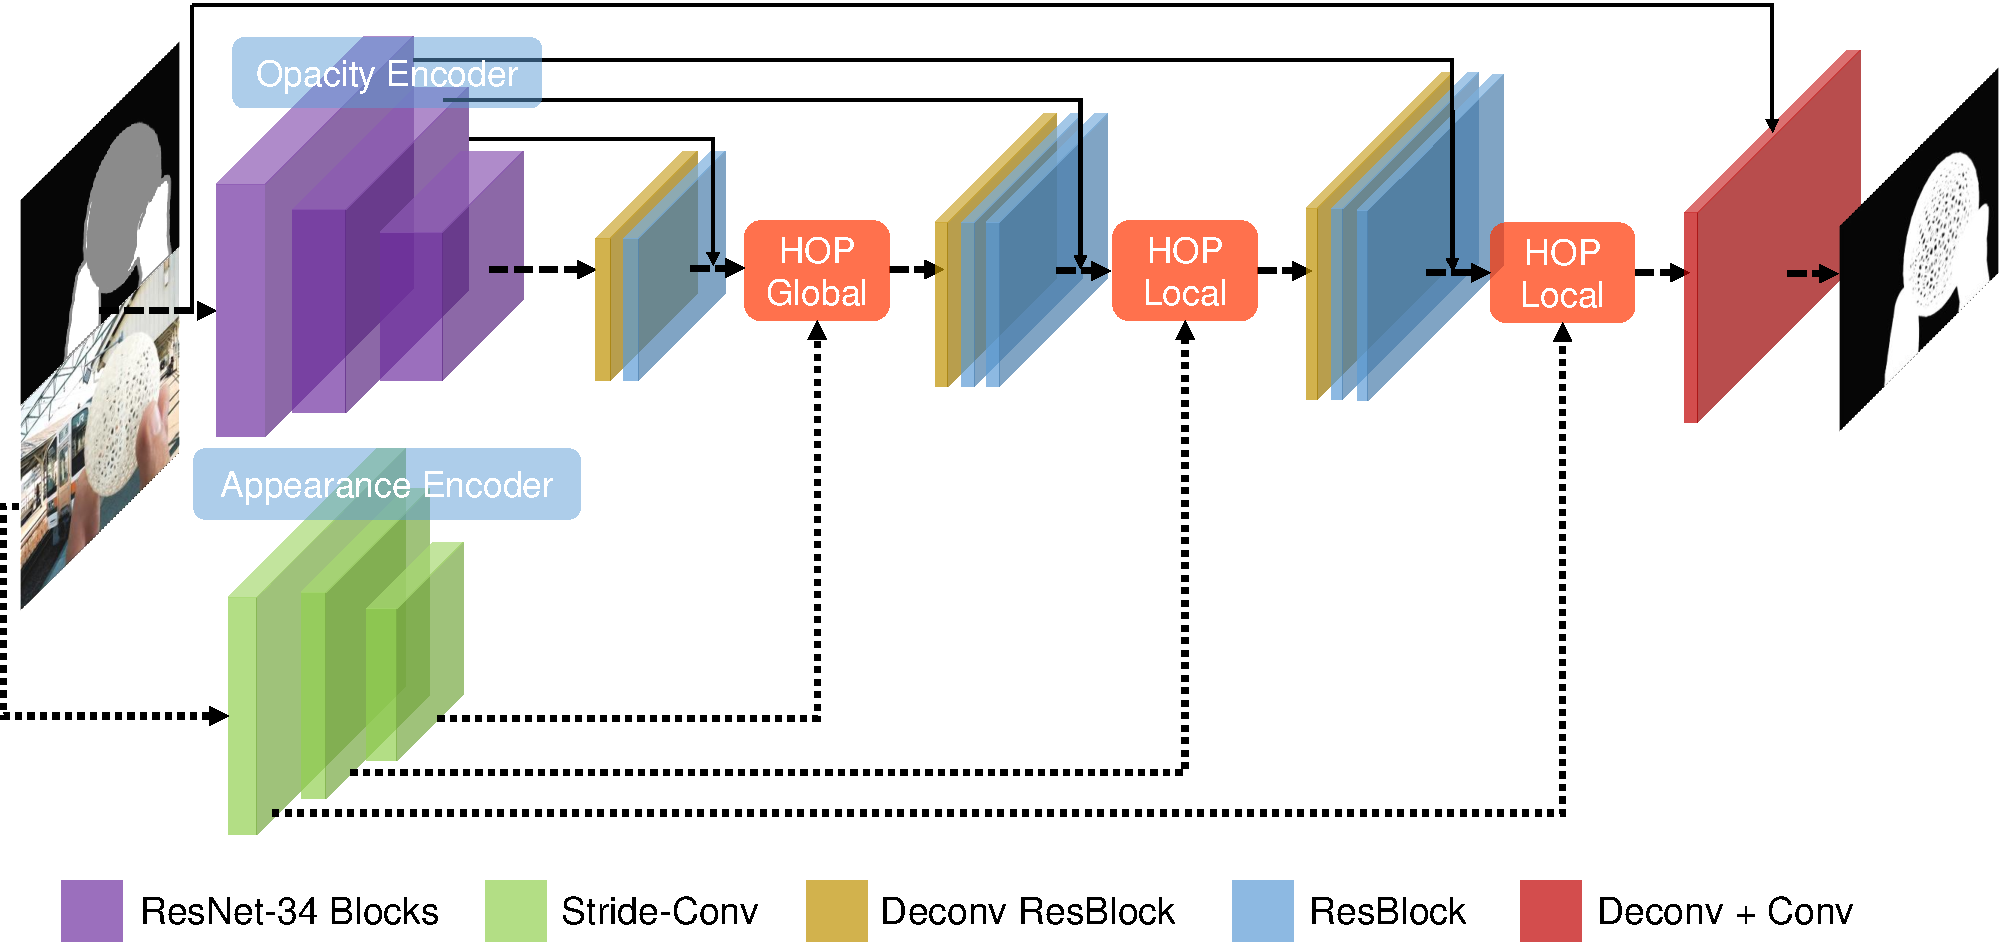
\includegraphics[width=0.66\linewidth]{chap5/arch.pdf}
		\label{fig5:diaga}
	}
	\centering	 
	\subfloat[]{
		\centering
		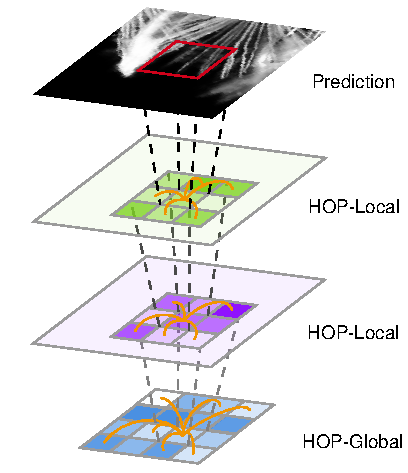
\includegraphics[width=0.33\linewidth]{chap5/diagram.pdf}
		\label{fig5:diagb}
	}
	\bicaption{所提出的HOP结构示意图。为了便于表示,图中仅示出了具有4个尺度等级的解码器和2个局部HOP模块。在具体实现中,网络模型具有包含5个尺度等级解码器和3个局部HOP块。(a)所提出的网络架构,外观编码器分支仅将RGB图像作为输入;(b)在不同语义级别的特征图上层次化不透明度传播的示意图,橙色线表示特征的传播}{Diagrams of our proposed HOP structure. For the ease of representation, only a 4-scale-level decoder and 2 local HOP blocks are shown. In our implementation, we have a 5-level decoder and 3 local HOP blocks. (a) The architecture of our network. The appearance encoder branch only takes RGB image as the input. (b) The schematic diagram of hierarchical opacity propagation on feature maps from different semantic level. Orange lines indicate the feature propagation}
	\label{fig5:diag}
\end{figure}

\subsection{层次化不透明度传播模块}
通常情况下,Non-local模块\cite{wang2018non}或Transformer\cite{vaswani2017attention}能够通过其中的自注意力机制(self-attention mechanism)\cite{lin2017structured}进行全局信息传播。但是,如果直接在自然图像抠像方法中采用原始的Non-local模块或图像Transformer,则会存在两个严重的缺陷。一方面,Non-local模块在计算代价很高,因此GCA Matting仅在特征尺寸较小的部分使用了与其相似的GCA机制。尽管为了减少计算量和内存消耗,有一些改进方法被提出\cite{zhu2019asymmetric},但对图像抠图这种需要在大尺寸特征图上进行不透明度信息传播的问题而言,依然不可行。另一方面,Non-local模块和Transformer都在唯一的输入特征图上构建一个完全图,并且完全图中边的权重是由节点的特征生成。在图像抠图任务中,每个节点的特征是不透明度信息。在某些语义任务(例如视频分类\cite{wang2018non},语义分割\cite{zhu2019asymmetric}或图像补全\cite{yu2018generative})中,基于不同特征节点之间的相似性传播语义特征相对而言非常直观且可行,而在自然图像抠图任务中传播过程需要更多的无语义的外观信息,而不是语义信息。


\begin{figure}[t]
	\centering
	\bisubcaptionbox{局部HOP模块\label{fig5:blocka}}%
					{local HOP block}
					[0.45\textwidth]{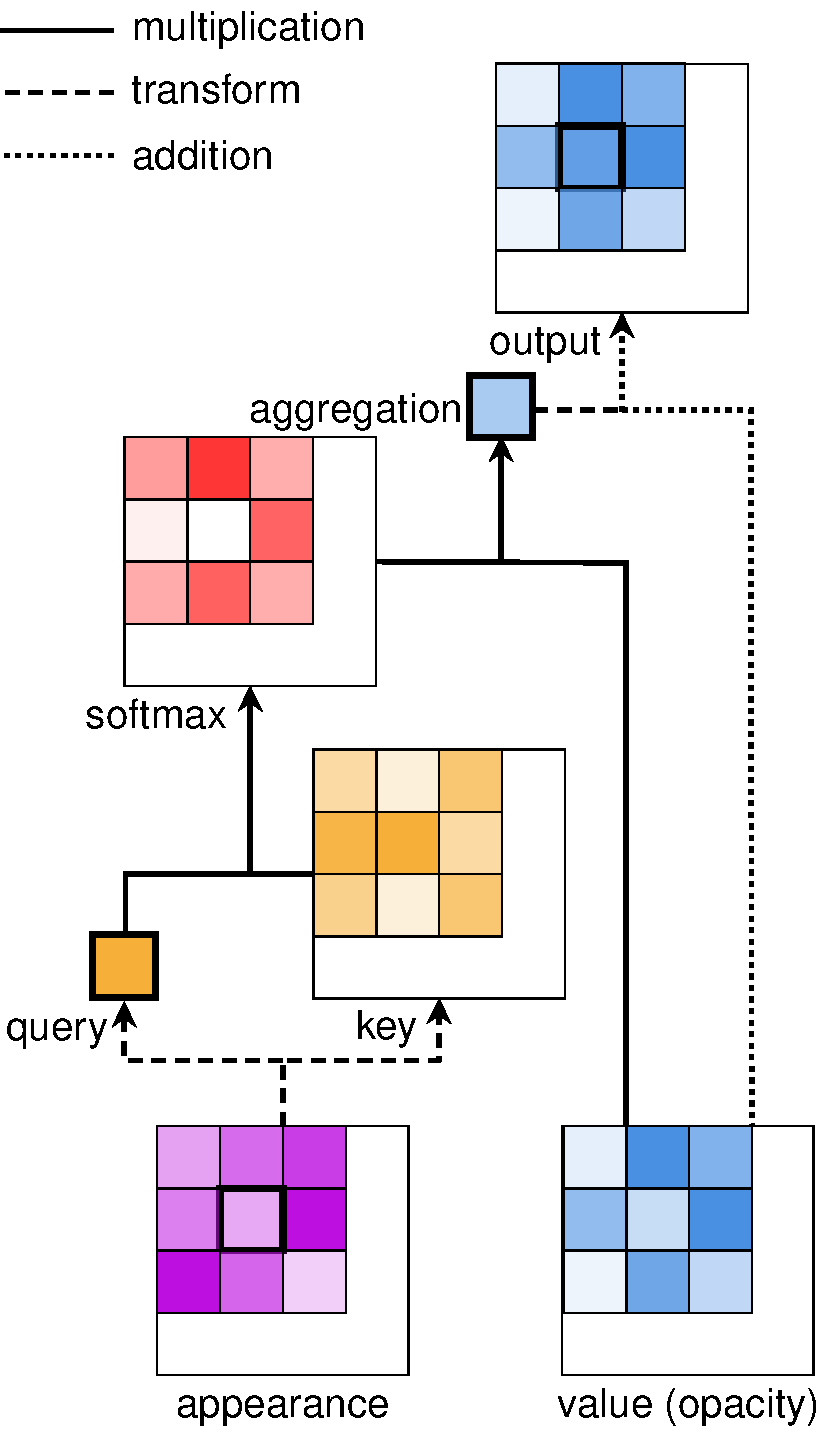
\includegraphics[height=.65\textwidth]{chap5/HOP-local.pdf}}
	\bisubcaptionbox{局部自注意力\label{fig5:blockb}}%
					{local self-attention}
					[0.45\textwidth]{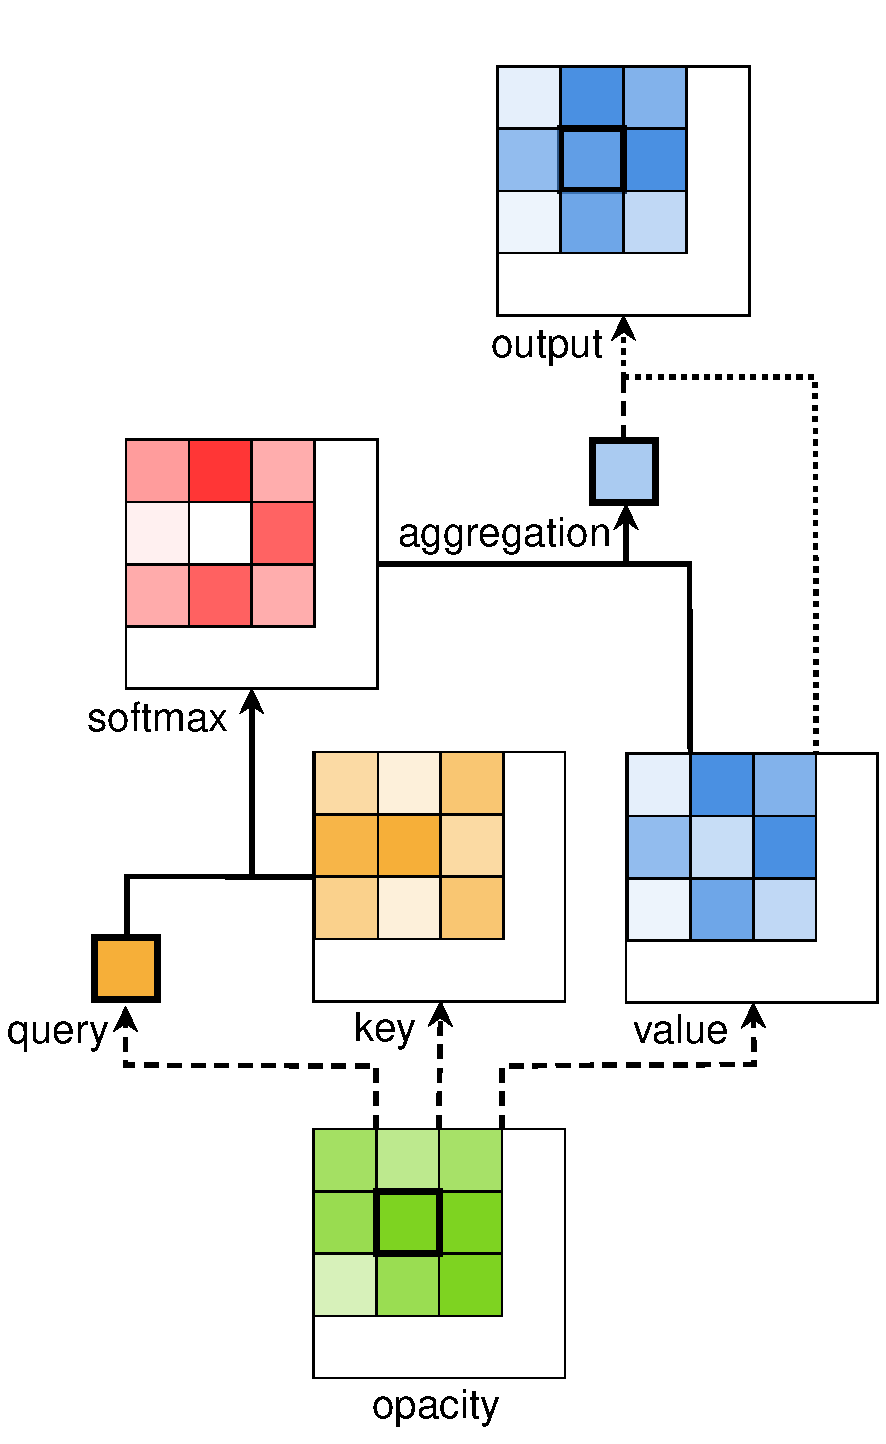
\includegraphics[height=.65\textwidth]{chap5/SA-local.pdf}}  
					                
	\centering
	\bisubcaptionbox{全局HOP模块\label{fig5:blockc}}%
					{global HOP block}
					[0.45\textwidth]{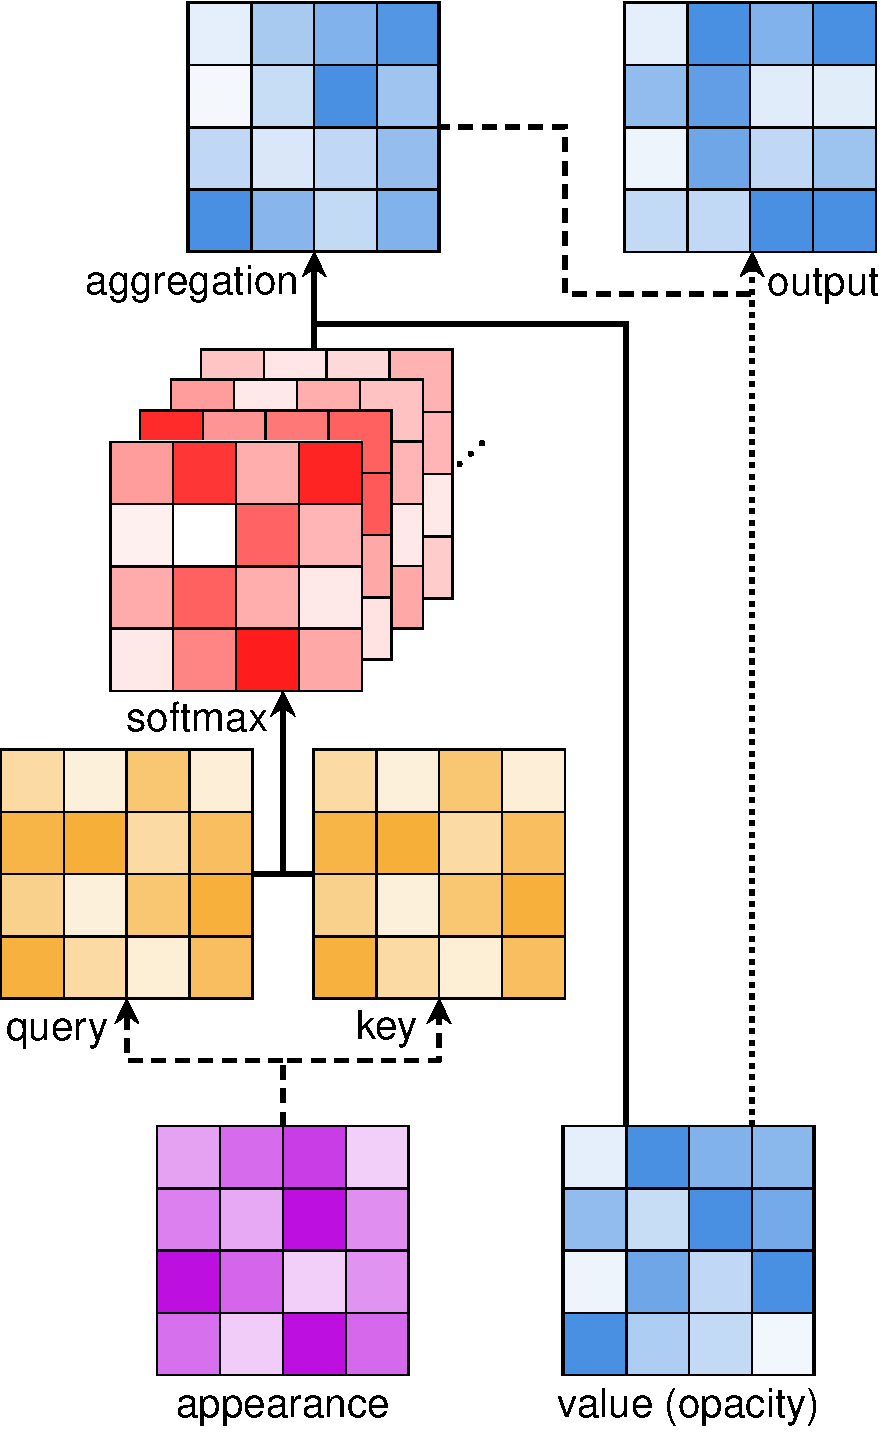
\includegraphics[height=.65\textwidth]{chap5/HOP-global.pdf}}
	\bisubcaptionbox{全局自注意力\label{fig5:blockd}}%
					{global self-attention}
					[0.45\textwidth]{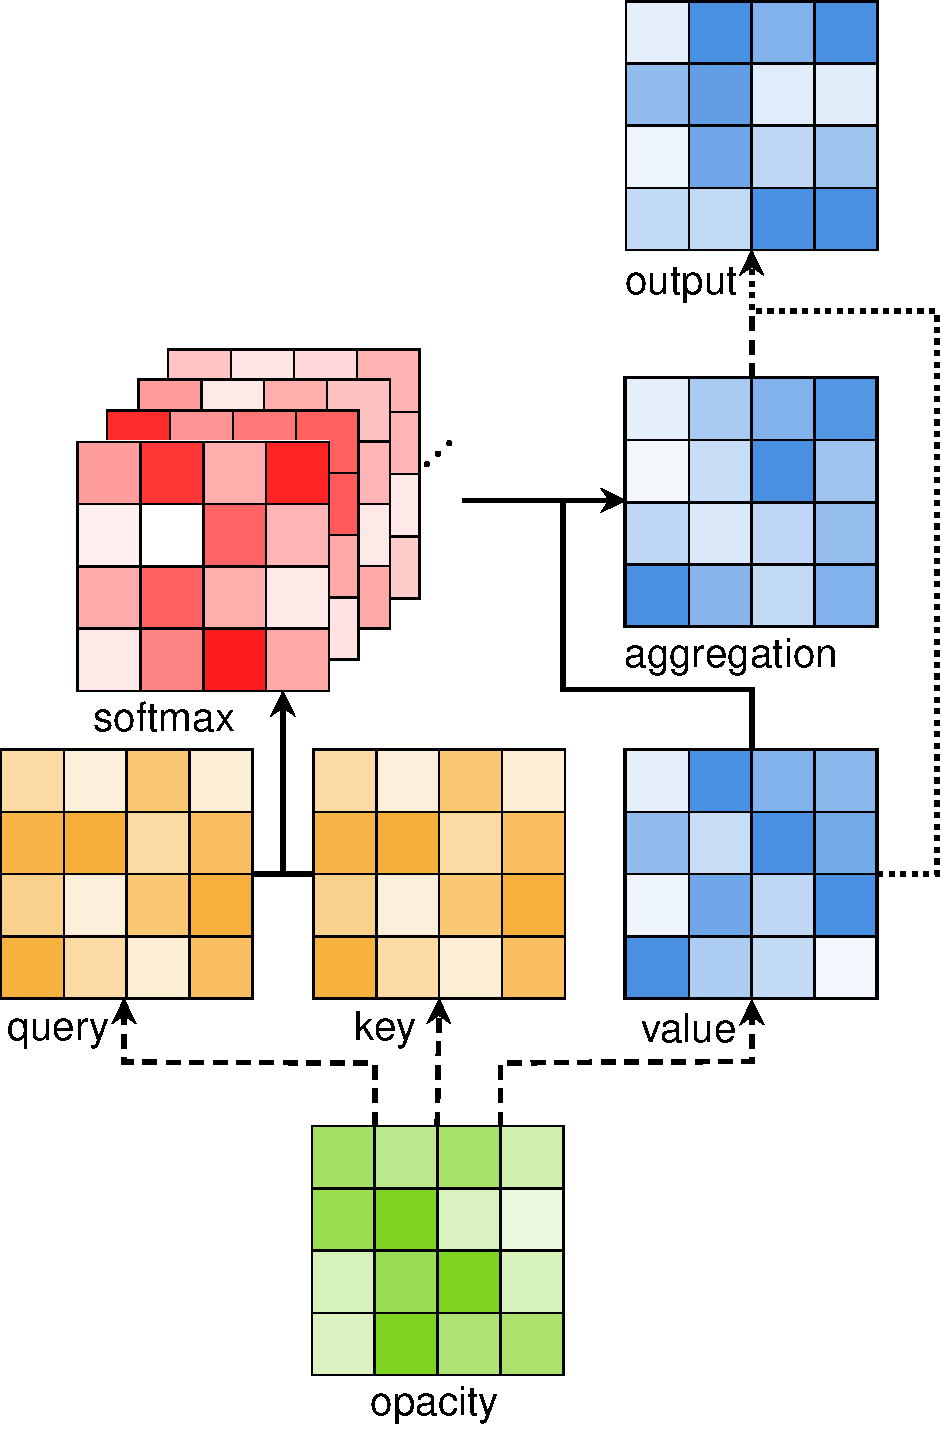
\includegraphics[height=.65\textwidth]{chap5/SA-global.pdf}}
	\bicaption{局部HOP模块、局部自注意力、全局HOP模块和全局自注意力的细节结构示意图,在两个局部模块示意图上为便于表示,仅展示了一个查询数据点}{The diagrams of detailed structure of local HOP block, local self-attention block, global HOP block and global self-attention block. For these two local blocks, we only show one query data point in the diagrams for the ease of presentation}
	\label{fig5:block}
\end{figure}

受到近期稀疏Transformer\cite{child2019generating,huang2019interlaced}和局部自注意力\cite{ramachandran2019stand}的成功的启发,在GCA Matting模型基础上,本节所提出的层次化不透明度传播结构包含了两种不同的传播模块,即全局HOP模块和局部HOP模块,两种模块在传播中同时利用了图像外观信息和不透明度预测信息。

所提出的HOP Matting的网络总体结构如图\ref{fig5:diaga}中所示。在该方法中,延续了GCA Matting模型的设计,具有两个编码器分支,一个作为不透明信息来源(即alpha遮罩信息),另一个作为图像外观信息来源。而全局HOP模块采用了GCA模块相同的构造形式,为便于下文中局部HOP模块的理解,在本节中,我们采用与注意力机制相似的数学形式重新对其进行定义。假设源自不透明度编码器和外观编码器的特征图分别被表示为$F^O\in\mathbb{R}^{HW\times C}$ 和$F^A\in\mathbb{R}^{HW\times C}$,特征图上位于 $(i,j)$的特征点为$f^O_{(i,j)}\in\mathbb{R}^{C}$和$f^A_{(i,j)}\in\mathbb{R}^{C}$,则全局HOP模块可定义为:
\begin{equation}
\begin{aligned}
q_{(i,j)} =& W_{QK}f^A_{(i,j)},\\ 
k_{(x,y)} =& W_{QK}f^A_{(x,y)}, \\
a_{(i,j),(x,y)} =& \mathop{\mathrm{softmax}}_{(x,y)}(\frac{q_{(i,j)}^Tk_{(x,y)}}{\|q_{(i,j)}\|\|k_{(x,y)}\|}),\\
g_{(i,j)} =& W_{out}(\sum_{(x,y)}a_{(i,j),(x,y)}f^O_{(x,y)}) + f^O_{(i,j)},
\end{aligned}
\end{equation}
其中$W_{QK}$为作用在键(key)与查询(query)上的线性变换,$W_{out}$ 是用于将传播后的信息与输入特征图$F^O$对齐的变换。此外,$F^O$在此处是不进行任何变换的注意力机制中的值(value)项,同时也可以将$v_{(x,y)}=W_{out}f^O_{(x,y)}$作为值项。图\ref{fig5:blockc}展示了全局HOP模块的结构细节。

不同于自注意力\cite{lin2017structured,vaswani2017attention}或者传统注意力机制\cite{bahdanau2014neural,xu2015show},在全局HOP模块中键和值是异源生成的。在自注意力机制中,查询、键和值都是从同一个特征中生成的,而在传统注意力机制中键和值也具有相同的信息来源。但是在HOP模块中,采用了GCA模块的思路,查询和键具有相同图像外观特征作为信息来源,而值项则以不透明度特征作为信息来源。

类似地,我们可以对只关注每个特征点的局部邻域的局部HOP模块进行公式化:
\begin{equation}
\begin{aligned}
a_{(i,j),(x,y)} = &\mathop{\mathrm{softmax}}_{(x,y)\in\mathcal{N}((i,j), s)}(\frac{q_{(i,j)}^Tk_{(x,y)}}{\|q_{(i,j)}\|\|k_{(x,y)}\|}),\\
g_{(i,j)} = &W_{out}(\sum_{(x,y)\in\mathcal{N}((i,j), s)}a_{(i,j),(x,y)}f^O_{(x,y)})\\& + f^O_{(i,j)},
\end{aligned}
\end{equation}
其中,$\mathcal{N}((i,j), s)$表示位于$(i,j)$特征点的窗口大小为$s$的空间近邻特征点集合。两种HOP模块与自注意力的区别可以从图\ref{fig5:gca_comp}或图\ref{fig5:block}中看出,在消融研究中,我们将所提出的两种HOP模块与全局/局部自注意力模块进行了性能对比。

利用前文所述的两种HOP模块,如图\ref{fig5:diagb}所示,我们构建了用于alpha遮罩值估计的完整的层次化不透明度传播(HOP)结构。一个HOP结构包括一个全局HOP模块和多个局部HOP模块。在示意图\ref{fig5:diagb}中,我们省略了HOP模块之间的卷积与反卷积层,以更清晰地显示如何层次化传播不透明度信息。底部的全局HOP模块将从神经网络的瓶颈处的特征图上进行全局的不透明度传播,该层次的特征图包含更多的语义信息但只有较少的纹理消息。
通过进行全局地语义特征传播以利用整个图像上全部的信息是一个非常直观的操作。随后,将局部HOP模块加入到网络中不同的反卷积阶段之间,在这些高分辨率特征图中存在更多的纹理表示信息。因此,这也促使了局部HOP模块仅需要关注每个查询点的空间局部近邻,以提取纹理信息。借助HOP结构,不透明度alpha特征可以在不同的特征级别上进行信息传播,先在语义特征上传播再到在纹理特征上传播,先在低分辨率特征图传播再到在高分辨率特征图上传播。

此外,所提出的HOP结构可以被视为一个4层的图卷积网络\cite{kipf2016semi},每层具有权重值不同的图结构,并且由于特征图的尺寸在变化,所以节点的数量在网络的不同阶段也是可变的。全局HOP模块中的图为完全图,而局部HOP模块中的相似性图是稀疏的。所有边权重均通过注意力机制进行计算,类似于图注意力网络(Graph Attention Networks,GATs)\cite{velivckovic2017graph}。

\subsection{位置编码}
在先前的一些工作中,自注意力机制中的位置编码总能带来一定的收益\cite{vaswani2017attention,dai2019transformer,ramachandran2019stand}。在本节中我们将对所提出的方法中加入的位置编码进行描述。我们采用两种不同的位置编码方式:全局HOP模块的尺度不敏感位置编码(scale-insensitive positional encoding)和局部HOP块的局部相对位置编码(local relative position encoding)。图\ref{fig5:PE}对不同的位置编码方法进行了展示。

\begin{figure}[t]
	% \subfloat{
	% 	\centering
	% 	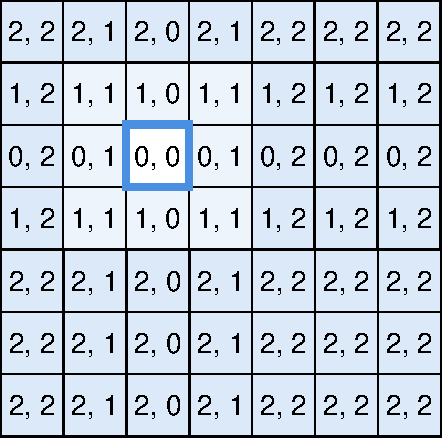
\includegraphics[width=.40\linewidth]{chap5/pos-scale.pdf}\\
	% 	\centering SI-PE
	% }	
	% \subfloat{
	% 	\centering
	% 	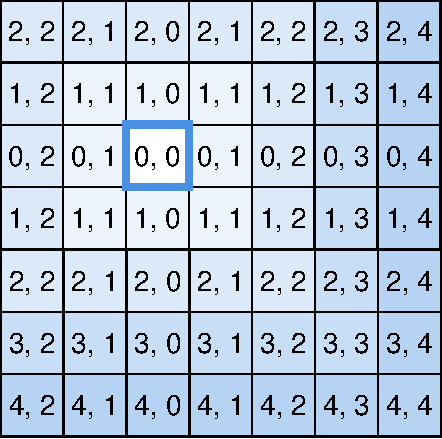
\includegraphics[width=.40\linewidth]{chap5/pos-relate.pdf}\\
	% 	\centering R-PE
	% }	

	% \subfloat{
	% 	\centering
	% 	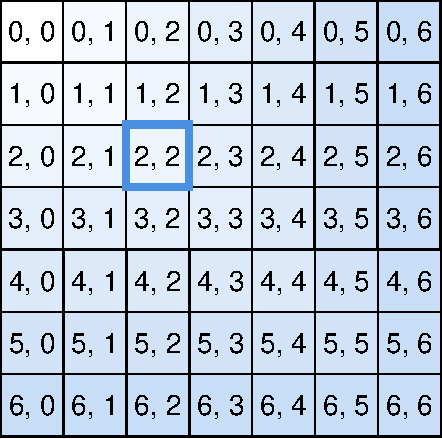
\includegraphics[width=.40\linewidth]{chap5/pos-abs.pdf}\\
	% 	\centering A-PE
	% }	
	% \subfloat{
	% 	\centering
	% 	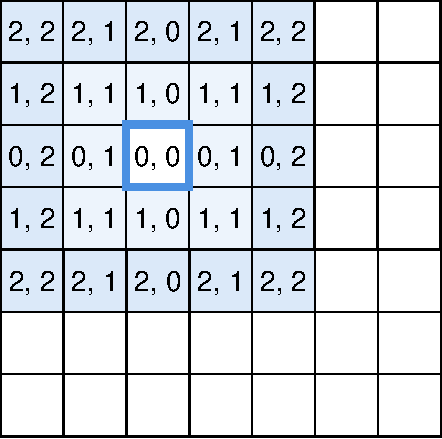
\includegraphics[width=.40\linewidth]{chap5/pos-local.pdf}\\
	% 	\centering LR-PE
	% }
	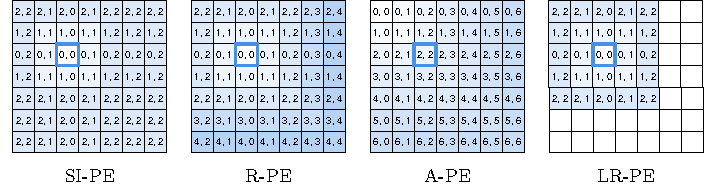
\includegraphics[width = 1\columnwidth]{chap5/pos_enc.pdf}
	\bicaption{不同的位置编码示意图。蓝色方框表示查询点的位置。每个特征点上的有序数对表示(行偏移,列偏移)。SI-PE:尺度不敏感位置编码;R-PE:相对位置编码;A-PE:绝对位置编码;LR-PE:局部相对位置编码}{The illustration of different positional encoding methods. The blue rectangle indicates the position of query. The ordered pair in each feature point is (row offset, column offset). SI-PE: scale-insensitive positional encoding; R-PE: relative positional encoding; A-PE: absolute positional encoding; LR-PE: local relative positional encoding}
	\label{fig5:PE}
\end{figure}

\subsubsection{尺度不敏感位置编码}
Vaswani等人\cite{vaswani2017attention}在自然语言处理任务中将位置编码引入Transformer以提升其性能。Transformer-xl \cite{dai2019transformer} 进一步将绝对位置编码扩展到相对位置编码。直觉上,我们可以将编码分为行编码和列编码,以将一维的相对或绝对位置编码扩展为用于图像抠图的二维位置编码。但是,已有的位置编码方式的严重的问题是注意力机制中的邻域大小必须固定。一旦输入图像的尺寸大于训练图像的尺寸,就会有一些在训练中从未出现过的位置编码,这使得测试过程变得不可行。在图像抠图中,测试图像大于训练所用图像区块的情况是非常常见的。为解决这个问题,我们为全局HOP模块提出了对尺度变化不敏感的位置编码。

在所提出的尺度不敏感位置编码中,定义空间近邻半径$s$。任意点超出半径的特征点共享完全相同的位置编码,而在半径$s$的特征点则采用相对位置编码。则带有该位置编码的全局HOP模块可以写为
\begin{equation}
\begin{aligned}
e_d =& \begin{cases} W_{PE}\,r_d  \quad d\le s;\\ W_{PE}\,r_s   \quad otherwise,\end{cases} \\
a_{(i,j),(x,y)} =& \mathop{\mathrm{softmax}}_{(x,y)}(\frac{q_{(i,j)}^Tk_{(x,y)}}{\|q_{(i,j)}\|\|k_{(x,y)}\|}\\ & + \frac{q_{(i,j)}^T}{\|q_{(i,j)}\|}(e_{|i-x|}+e_{|j-y|})),\\
g_{(i,j)} =& W_{out}(\sum_{(x,y)}a_{(i,j),(x,y)}f^O_{(x,y)}) + f^O_{(i,j)},
\end{aligned}
\end{equation}
式中我们延续文献\parencite{vaswani2017attention,dai2019transformer}的设定采用正弦编码,并在实现中采用$s=7$。借助尺度不敏感位置编码,所提出的HOP Matting方法能够处理任意形状和尺度的输入图像。除位置编码外,我们还设计了trimap图编码,以学习在注意力机制中是否需要给前景、背景和位置区域设置不同的权重。因此$(e_{|i-x|}+e_{|j-y|})$项可以被改进为$(e_{|i-x|}+e_{|j-y|}+W_{T}t_{(x,y)})$,其中$t_{x,y}$是在缩放后的trimap图中位置$(x,y)$的数据点。

\subsubsection{局部相对位置编码}
对于局部HOP模块,邻域大小在网络中始终是一个常数,这使得其并不需要尺度不敏感位置编码。
我们将文献\parencite{ramachandran2019stand}中提出的局部相对位置编码扩展为具有方向不变性(direction-invariant)的版本,而没有提出新的编码方式。局部HOP模块中的位置编码方式如图\ref{fig5:PE}中LR-PE所示。

与先前工作中所用的位置编码\cite{vaswani2017attention,dai2019transformer,ramachandran2019stand}形成对比,我们的图像抠图方法采用的位置编码都是具有方向不变性的,这意味着编码仅与查询和键之间的绝对距离有关,而和两者之间相对的方向位置无关。这种特性源自于自然图像抠图属于语义层次较低的低级视觉问题,所以应该具有旋转不变性(rotation-invariant)。

\subsection{神经网络实现细节}

在该网络模型的训练中,我们依然延续了基线网络模型的训练设定。损失函数采用了公式(\ref{eq5:loss})中的alpha预测损失,仅在trimap图标注的位置区域对预测结果和真实标注计算平均L1损失。对于不透明度编码器,我们使用了在ImageNet数据集\cite{russakovsky2015imagenet}上预训练的ResNet-34网络\cite{he2016deep}的前11个模块。而对于图像外观编码器,我们只选择了步长为2的卷积层进行堆叠,以抽取尽可能低级的图像特征。

网络模型使用Adobe Image Matting数据集\cite{xu2017deep}的前景图片和MS COCO数据集中的背景图片进行训练\cite{lin2014microsoft}。在基本数据增广部分延续了第\ref{sec5:aug}节中描述的数据增广方式,在基本增广部分之外还引入了有效的随即插值(Random Interpolation,RI)增广方式,我们将在第\ref{sec5:RI}节中对该数据增广方式及其有效性进行详细讨论。在训练时同时使用了批归一化\cite{ioffe2015batch}和谱归一化\cite{miyato2018spectral}对训练过程进行归一化操作。采用Adam优化器\cite{kingma2014adam}实现网络参数优化。同时参考文献\parencite{he2019bag},采用FP16半精度方式进行网络的训练以节约显存空间。在学习率方面,采用了学习率预热\cite{goyal2017accurate}及余弦衰减\cite{loshchilov2016sgdr}策略。

在表\ref{tab5:arch}中我们给出了所提出的HOP Matting网络模型的结构细节。我们在表\ref{tab5:arch}中忽略了全局和局部HOP模块中的线性变换层,以使表格保持简洁。全局和局部HOP模块中的线性变换均采用卷积核为$1\times 1$的卷积层,且输入通道数与输出通道数相等。在除Decoder-Stage-5中最后一个卷积层之外,我们对表\ref{tab5:arch}中所描述的所有卷积层均采用了批归一化\cite{ioffe2015batch}和谱归一化\cite{miyato2018spectral}处理。在算法\ref{alg5:local}中我们提供了一种可以用于实现局部HOP模块的PyTorch\cite{paszke2017automatic}风格伪代码。在该伪代码中,我们同样地省略了线性变换操作。

\begin{table}
	\bicaption{所提出的HOP Matting网络的结构细节}{Detailed structure of the proposed HOP Matting network}
	\centering
	\label{tab5:arch}
	\begin{tabular}{|Sc|Sc|Sc|Sc|Sc|Sc|Sc|}
		\hline
		\multirow{15}{*}{Encoder} & \multicolumn{3}{c|}{Opacity Encoder} & \multicolumn{3}{c|}{Appearance Encoder} \\ 
		\cline{2-7} 
		& Stage  & Output Size &  & Stage  & Output Size &  \\ 
		\cline{2-7} 
		& \multirow{2}{*}{Stage 1} & \multirow{2}{*}{256$\times$256} & $\text{conv}$, 3$\times$3, 32, stride 2 & \multirow{2}{*}{Stage 1} & \multirow{2}{*}{256$\times$256} & \multirow{2}{*}{$\text{conv}$, 3$\times$3, 16} \\ 
		% 		\cline{4-4}
		&  &  & $\text{conv}$, 3$\times$3, 32 &  &  &  \\ \cline{2-7} 
		& \multirow{3}{*}{Stage 2} & \multirow{3}{*}{128$\times$128} & $\text{conv}$, 3$\times$3, 64, stride 2 & \multirow{3}{*}{Stage 2} & \multirow{3}{*}{128$\times$128} & \multirow{3}{*}{$\text{conv}$, 3$\times$3, 32} \\
		% 		\cline{4-4}
		&  &  & $\begin{bmatrix} \text{conv},& 3\times3,& 64 \\ \text{conv},&3\times3,& 64 \end{bmatrix}\times 3$ &  &  &  \\ \cline{2-7}
		& Stage 3 & 64$\times$64 & $\begin{bmatrix}\text{conv},&3\times3,&128 \\ \text{conv},&3\times3,&128 \end{bmatrix}\times 4$ & Stage 3 & 64$\times$64 &$\text{conv}$, 3$\times$3, 64 \\ \cline{2-7} 
		& Stage 4 & 32$\times$32 & $\begin{bmatrix} \text{conv},&3\times3,& 256 \\ \text{conv},&3\times3,& 256\end{bmatrix}\times 4$ & Stage 4 & 32$\times$32 & $\text{conv}$, 3$\times$3, 64 \\ \cline{2-7} 
		& Stage 5 & 16$\times$16 & $\begin{bmatrix} \text{conv},&3\times3,& 512\\ \text{conv},&3\times3,& 512 \end{bmatrix}\times 2$ &  &  &  \\ \hline\hline
		\multirow{25}{*}{Decoder} & \multicolumn{2}{c|}{Stage } & \multicolumn{1}{c|}{Output Size} & \multicolumn{3}{c|}{} \\ \cline{2-7} 
		& \multicolumn{2}{c|}{\multirow{4}{*}{Stage 1}} & \multicolumn{1}{c|}{\multirow{4}{*}{32$\times$32}} & \multicolumn{3}{Sc|}{$\begin{bmatrix} \text{deconv},&4\times4,&256\\ \text{conv},&3\times3,&256\end{bmatrix}$} \\ 
		% 		\cline{6-7} 
		& \multicolumn{2}{c|}{} & \multicolumn{1}{c|}{} & \multicolumn{3}{Sc|}{$\begin{bmatrix} \text{conv},&3\times3,&256\\ \text{conv},&3\times3,&256\end{bmatrix}$}\\
		& \multicolumn{2}{c|}{} & \multicolumn{1}{c|}{} & \multicolumn{3}{c|}{global HOP}\\ \cline{2-7} 
		& \multicolumn{2}{c|}{\multirow{4}{*}{Stage 2}} & \multicolumn{1}{c|}{\multirow{4}{*}{64$\times$64}} & \multicolumn{3}{Sc|}{$\begin{bmatrix} \text{deconv},&4\times4,&128\\ \text{conv},&3\times3,&128\end{bmatrix}$} \\ 
		% 		\cline{6-7} 
		& \multicolumn{2}{c|}{} & \multicolumn{1}{c|}{} & \multicolumn{3}{Sc|}{$\begin{bmatrix} \text{conv},&3\times3,&128\\ \text{conv},&3\times3,&128\end{bmatrix} \times 2$} \\
		& \multicolumn{2}{c|}{} & \multicolumn{1}{c|}{} & \multicolumn{3}{c|}{local HOP} \\ \cline{2-7} 
		& \multicolumn{2}{c|}{\multirow{4}{*}{Stage 3}} & \multicolumn{1}{c|}{\multirow{4}{*}{128$\times$128}} & \multicolumn{3}{Sc|}{$\begin{bmatrix} \text{deconv},&4\times4,&64 \\ \text{conv},&3\times3,&64\end{bmatrix} $} \\ 
		% 		\cline{6-7} 
		& \multicolumn{2}{c|}{} & \multicolumn{1}{c|}{} & \multicolumn{3}{Sc|}{$\begin{bmatrix} \text{conv},&3\times3,&64 \\ \text{conv},&3\times3,&64\end{bmatrix} \times 2 $} \\
		& \multicolumn{2}{c|}{} & \multicolumn{1}{c|}{} & \multicolumn{3}{c|}{local HOP} \\ \cline{2-7} 
		& \multicolumn{2}{c|}{\multirow{4}{*}{Stage 4}} & \multicolumn{1}{c|}{\multirow{4}{*}{256$\times$256}} & \multicolumn{3}{Sc|}{$\begin{bmatrix} \text{deconv},&4\times4,&32\\ \text{conv},&3\times3,&32\end{bmatrix} $} \\ 
		% 		\cline{6-7} 
		& \multicolumn{2}{c|}{} & \multicolumn{1}{c|}{} & \multicolumn{3}{Sc|}{$\begin{bmatrix} \text{conv},&3\times3,&32\\ \text{conv},&3\times3,&32\end{bmatrix} $} \\
		& \multicolumn{2}{c|}{} & \multicolumn{1}{c|}{} & \multicolumn{3}{c|}{local HOP} \\ \cline{2-7} 
		& \multicolumn{2}{c|}{\multirow{2}{*}{Stage 5}} & \multicolumn{1}{c|}{\multirow{2}{*}{512$\times$512}} & \multicolumn{3}{Sc|}{$\text{deconv}$,  4$\times$4,  32,  $\text{stride }$2} \\ 
		% 		\cline{6-7} 
		& \multicolumn{2}{c|}{} & \multicolumn{1}{c|}{} & \multicolumn{3}{Sc|}{$\text{conv}$,  3$\times$3,  32} \\ \hline
	\end{tabular}
\end{table}
	

\begin{algorithm}[h]
	\SetKwInput{KwIn}{输入}
	\SetKwInput{KwOut}{输出}
	\caption{局部HOP模块的PyTorch风格伪代码}
	\label{alg5:local}
	\KwIn{外观特征张量 $F: N\times C\times H\times W$;不透明度特征张量 $A: N\times C'\times H\times W$;局部相关性窗口大小 $k$。 }
	\KwOut{传播后的alpha特征张量 $A': N\times C'\times H\times W$。}
	$R\gets \mathrm{ReflectPadding}(F, \lfloor k/2\rfloor)$ \;
	$R\gets \mathrm{Unfold}(R, k)$; \qquad\qquad\qquad\qquad\# $R: [N, Ck^2, HW]$\\
	$R\gets \mathrm{Reshape}(R, [N,C,k^2,H,W])$\;
	$F\gets \mathrm{Repeat}(F, [1,1,k^2,1,1])$; \qquad\quad\# $F:[N, C, k^2, H, W]$\\
	\nonl \# \textit{计算相关性} $C$ \\
	$C\gets \mathrm{ReduceSum}(F\circ R,  \mathrm{dim}=1)$; \quad\# $C: [N,1,k^2,H,W]$\\
	$S\gets \mathrm{SoftMax}(C, \mathrm{dim}=2)$; \qquad\quad\:\:\:\,\, \# $S:[N,1,k^2,H,W]$\\
	\nonl \# \textit{传播}\\
	$A\gets \mathrm{ReflectPadding}(A, \lfloor k/2\rfloor)$ \;
	$A\gets \mathrm{Unfold}(A, k)$; \qquad\qquad\qquad\qquad\# $A: [N, C'k^2, HW]$\\
	$A\gets \mathrm{Reshape}(A, [N,C',k^2,H,W])$\;
	$A'\gets \mathrm{ReduceSum}(S\circ A, \mathrm{dim}=2)$; \quad \# $A': [N,C',H,W]$
\end{algorithm}


\section{实验结果}
为证明所提出方法的有效性,在本节中对所提出的两种方法进行了大量的实验,并针对HOP Matting方法设计了大量的消融实验。我们在两个被广泛使用的数据集上报告了所提出算法的评测结果:Composition-1k测试集\cite{xu2017deep}和alphamatting.com数据集\cite{rhemann2009perceptually}。在评估测度方面遵循文献\parencite{rhemann2009perceptually}的建议,采用均方误差(Mean Square Error,MSE)、总绝对差(Sum of Absolute Difference,SAD)、梯度误差(Gradient error,Grad)和连通误差(Connectivity error,Conn)对实验结果进行评估。为方便理解网络模型信息传播部分的作用,本节中将对所提两种模型的注意力机制部分进行可视化。


\begin{table}[t]
	\setlength{\tabcolsep}{15pt}
	\bicaption{使用不同测试时插值算法对Composition-1k测试集调整图片大小后的评估结果。RI表示随机插值增广}{Evaluation results on the resized Composition-1k testing set with different testing interpolations. RI is for random interpolation augmentation}
	\centering
	%    
	\begin{tabular}{l|cccc}  
		\toprule
		Methods & Test Interp.& SAD & MSE($10^{-3}$)  & Grad\\
		\midrule
		\multirow{3}{*}{ground-truth}&nearest& 21.66& 6.6& 13.76 \\
		& bilinear&5.8& 0.4&0.49 \\
		& cubic & 1.1& 0.02& 0.02\\
		\midrule
		\multirow{3}{*}{IndexNet Matting \cite{lu2019indices}}&nearest& 62.43& 23.8& 42.91 \\
		& bilinear&46.35& 14.1&24.41 \\
		& cubic & 45.65& 13.1& 25.47\\
		\midrule
		\multirow{3}{*}{HOP-5x5}&nearest&63.79&25.4&39.85\\
		& bilinear & 49.71 & 19.2 & 27.41\\
		& cubic & 38.45& 11.2  &18.87\\
		\midrule
		\multirow{3}{*}{HOP-5x5 + RI}  &nearest& 53.99 &19.5  &40.81\\
		& bilinear &30.34&6.5 &12.87\\
		& cubic & \textbf{29.42} & \textbf{6.3}&\textbf{12.16}\\
		\bottomrule
	\end{tabular}
	\label{tab5:RI}
\end{table}

\subsection{随机插值增广}
\label{sec5:RI}
经验上,深度图像抠图方法的实际性能对输入图像的缩放非常敏感。这是因为典型的自然图像抠图方法会关注图像中的细节纹理信息,而缩放操作可能会使图像边缘或高频信息出现模糊,从而导致性能下降。因此,大多数抠图方法都在原始输入图像上进行测试评估,不进行任何缩放的操作。在Context-aware Matting\cite{hou2019context}中,作者声称不同图像格式的前景和背景图片会将细微人工合成痕迹引入到合成的训练图像中,这些人工合成痕迹可以帮助网络简单地区分前景和背景。类似地,在本节中,我们将展示一些新的观察结果,即基于深度神经网络的抠图方法对不同的插值算法具有敏感性,同时对所提出的HOP Matting方法中使用的随机插值(Random Interpolation,RI)增广进行介绍。

我们在Composition-1k测试集\cite{xu2017deep}设计了一个经验性实验来支撑所描述的观察结论。首先,通过一个选定的插值算法对RGB图像进行缩放系数为1.5的上采样,然后通过相同的插值算法对放大图像进行下采样使其回到原尺寸。具体地说,假设原输入RGB图像为$800 \times 800$,并且所选的测试用插值算法为双线性插值。则通过双线性插值将输入RGB图像的大小调整为$1200 \times 1200$,然后再通过双线性插值将缩放后图像的尺寸重新调整为$800\times 800$。最后,将缩放回原尺寸的RGB图像输入网络进行alpha遮罩值预测,并评估预测值与原始真实标注之间的误差。值得注意的是,本实验并不是先进行下采样再进行上采样操作,因为先进行下采样必然会导致大量的信息丢失,而先进行上采样在理想情况下可以不产生任何信息损失。


表\ref{tab5:RI}展示了该经验性实验的评估结果。在该实验中,我们提供\textit{ground-truth}方法作为对照参考。\textit{ground-truth}方法表示直接对真实标注进行上采样和下采样,而不通过缩放后的输入图像进行任何alpha遮罩估计,然后计算缩放回原尺寸的真实标注和未经过缩放操作的真实标注之间的误差。这些结果揭示了插值操作本身所引入的误差,可以将其视为这些评估结果的理想下界。\textit{HOP-5x5}方法将作为HOP Matting方法的基本模型出现在本节的实验中。\textit{HOP-5x5}表示在局部HOP模块中采用$5\times 5$的空间邻域,并且在所有HOP模块中没有使用位置编码或trimap编码。同时我们还提供了IndexNet Matting\cite{lu2019indices}方法的评估结果作为对照。

从表\ref{tab5:RI}中可以注意到,不同测试时插值算法之间的果差距大多数结都大于\textit{ground-truth}下限之间的差距。换句话说,与插值缩放操作本身相比,作用在输入图像上的不同插值算法会在预测中引入更多误差。同时还可以看到\textit{HOP-5x5}方法的双线性插值和三次样条插值结果之间的差距大于IndexNet Matting\cite{lu2019indices}方法所给出的结果。我们对此的解释是,在训练集的数据增广中,HOP Matting方法遵循Deep Matting\cite{xu2017deep}所提出的数据合成方式,通过三次样条插值将背景图像缩放为与前景相同的大小然后合成。这种固定算法的插值增广方式使HOP Matting的模型更适合处理三次样条插值生成的数据。

基于上述经验观察结果,我们将随机插值增广方式引入所提出的HOP Matting方法。在训练阶段的数据预处理中对于任何缩放操作,都依相同的概率在不同的插值算法中进行采样,并通过采样到的插值算法实现缩放。因此,在每一个批量(mini-batch)中的合成训练图可能是由不同的插值算法生成的。此外,在合成训练图之前,可以使用不同的插值算法对前景、背景和alpha遮罩图进行缩放。如表\ref{tab5:RI}所示,使用随机插值所进行的训练不仅可以提高整体性能,而且可以减小双线性插值和三次样条插值之间误差的差距。

\begin{figure}[t]
	\centering
	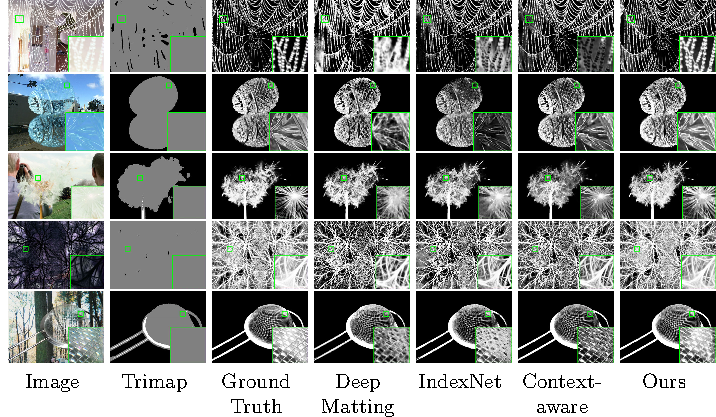
\includegraphics[width=1\textwidth]{chap5/adobe.pdf}
	\bicaption{在Composition-1k测试集\cite{xu2017deep}上的视觉效果对比结果}{The visual comparison results on Composition-1k testing set \cite{xu2017deep}}
	\label{fig5:adobe}
\end{figure}

\begin{table}[t]
	\setlength{\tabcolsep}{8pt}
	\bicaption{在Composition-1k测试集上的数值结果。PosE表示HOP模块中的位置编码,TriE表示HOP模块中的trimap编码,RI表示随机插值增广。本章所提出的不同模型变种用斜体表示,最佳数值结果加粗表示}{The quantitative results on Composition-1k testing set. PosE stands for positional encoding, and TriE is for trimap encoding in HOP blocks and RI for random interpolation augmentation. The variants of our approaches are emphasized in italic. Best results are in boldface.}
	\centering
	%    
	\begin{tabular}{l|cccc}  
		\toprule
		Methods & SAD & MSE($10^{-3}$) & Grad &Conn\\
		\midrule
		%		KNN Matting \cite{chen2013knn}& 175.4 & 103& 124.1 &176.4\\    
	%	Closed-Form Matting \cite{levin2008closed}& 168.1&91 &126.9& 167.9\\
		DCNN Matting\cite{cho2019deep}& 161.4& 87 &115.1& 161.9 \\
		Learning Based Matting \cite{zheng2009learning}&113.9& 48 &91.6 &122.2\\ 
		Information-flow Matting\cite{aksoy2017designing} & 75.4& 66& 63.0&-\\
		Deep Matting\cite{xu2017deep} &50.4& 14& 31.0& 50.8\\
		IndexNet Matting\cite{lu2019indices} &45.8&	13&	25.9&	43.7\\	
		AdaMatting\cite{cai2019disentangled}&41.7&10  &16.8 &-\\
		SampleNet Matting\cite{samplenet} &40.35&	9.9&	-&	-\\	
		Context-aware Matting\cite{hou2019context}& 35.8 & 8.2& 17.3& 33.2\\
		\midrule
		%		\textit{HOP-1x1} & 36.17& 9.1& 16.31& 33.72 \\  % & 42.53  & 40.84
		\textit{Baseline}  & 40.62 & 10.6 & 21.53 & 38.43\\
		\textit{GCA Matting} &35.28&	9.1&	16.92&	32.53\\
		\textit{HOP-5x5}& 34.82& 9.0 & 16.01& 32.04\\
		% 		\textit{HOP-5x5 + PosE}& 33.87& 8.2 & 15.34& 31.09\\
		% 		\textit{HOP-5x5 + PosE + TriE}& 34.15& 8.1 & 15.33& 31.45\\
		
		\textit{HOP-9x9}& {33.44}&{8.2}& {15.62}&{30.44} \\
		\textit{Baseline + RI}& 30.45& 6.8 & 13.23& 26.81\\
		\textit{HOP-5x5 + PosE + TriE + RI} & {28.12}& {5.8} & {11.36}& {24.13}\\
		\textit{HOP-9x9 + PosE + TriE + RI}& \textbf{27.80}& \textbf{5.7} & \textbf{11.25}& \textbf{23.73}\\
		\bottomrule
	\end{tabular}
	\label{tab5:adobe}
\end{table}
	

\subsection{Composition-1k测试集实验结果}
Composition-1k测试集\cite{xu2017deep}包含有50个不同的前景图生成的1,000张合成测试图。如表\ref{tab5:adobe}所示,本节对所提出的方法与当前最先进的自然图像抠图方法进行了定量比较。变体方法\textit{Baseline + RI}表示没有任何GCA模块或HOP模块的基线网络经过随机插值增广所训练出的网络模型。可以看出变体方法中的大多数都优于当前最先进的方法。在图\ref{fig5:adobe}中显示了Composition-1k测试集中一些测试结果的视觉效果对比。其中Deep Matting\cite{xu2017deep}的结果通过IndexNet Matting\cite{lu2019indices}中所提供的源代码和预训练模型生成。

此外,表\ref{tab5:eff}比较了一些最新方法的参数数量和模型效率。通过在具有11G显存的单个NVIDIA RTX 2080 Ti GPU上对Composition-1k测试集进行测试,该实验评估了每张测试图像的平均推理时间。值得注意的是,Context-aware Matting\cite{hou2019context}和Deep Matting\cite{xu2017deep}需要超过11G的显存或使用CPU计算,才能对Composition-1k测试集中的高分辨率图像估计其alpha遮罩值。因此,对于这两种方法,我们以缩放系数0.8对输入图像进行下采样后再进行测试。


\begin{table}[t]
	\setlength{\tabcolsep}{15pt}
	\bicaption{参数数量及使用单张NVIDIA RTX 2080 Ti显卡情况下在Composition-1k测试集上的测试效率对比。对于Deep Matting和Context-aware Matting方法,在原图基础上采用缩放系数0.8进行降采样后作为输入图片}{Parameter numbers and efficiency comparison on Composition-1k testing set on a single NVIDIA RTX 2080 Ti. Input images of Deep Matting and Context-aware Matting are downsampled with a factor of 0.8}
	\centering
	%    
	\begin{tabular}{l|cc}  
		\toprule
		Methods & \# of Parameters & Mean Time \\
		\midrule
		Deep Matting\cite{xu2017deep} &	130.6 M & 0.245 s \\
		Context-aware Matting\cite{hou2019context} & 107.5 M & 3.915 s\\
		IndexNet Matting\cite{lu2019indices} &	\textbf{6.0 M} &\textbf{ 0.182 s}\\	
		\midrule
		\textit{HOP-1x1} & 25.3 M & \textbf{0.182 s} \\
		\textit{HOP-5x5} & 25.3 M & 0.255 s \\
		\textit{HOP-9x9} & 25.3 M & 0.339 s \\
		\bottomrule
	\end{tabular}
	\label{tab5:eff}
\end{table}

\subsection{Alphamatting.com数据集实验结果}
alphamatting.com数据集被用于alphamatting在线评测排行榜,其中包含8张测试图片。每张测试图包含三种不同类型的trimap图,即小范围、大范围和用户标注。该排行榜首先对共计24个测试样例分别进行测试排名,然后再对每个类型trimap图下的8个测试样例排名取平均数,作为该类trimap图下的排名值,最后对所有测试样例的排名求取平均数,作为每个评测指标下的总排名成绩。表\ref{tab5:alphamatting}展示了所提出的两种方法在alphamatting.com排行榜中的平均排名值。每一个评估测度下的\textit{Overall}排名表示在三种类型trimap图上的所有排名名次的平均值。如表\ref{tab5:alphamatting}中排名结果所示,本章所提出的HOP Matting在不同评估测度下的表现均优于其他最先进方法,GCA Matting方法也优于多数最先进的抠图方法。

\begin{table}[t]
% \setlength{\tabcolsep}{2pt}
\bicaption{所提出两种模型在alphamatting.com排行榜上的排名得分。S、L和U分别表示排行榜测试集中三种trimap图的类型,即小范围、大范围和用户标注}{Our scores on the alphamatting.com benchmark. S, L and U denote three trimap types, small, large and user, included in the benchmark.}
\footnotesize
\centering
\begin{tabular}{@{\;\;}l|@{\;\;}c@{\;\;}|@{\;\;}c@{\;\;}c@{\;\;}c@{\;\;}|@{\;\;}c@{\;\;}|@{\;\;}c@{\;\;}c@{\;\;}c@{\;\;}|@{\;\;}c@{\;\;}|@{\;\;}c@{\;\;}c@{\;\;}c@{\;\;}}
	\toprule
	%		& \multicolumn{4}{c}{Average Rank}\\
	\multirow{2}{*}{Average Rank} & \multicolumn{4}{c@{\;\;}|@{\;\;}}{SAD}& \multicolumn{4}{c@{\;\;}|@{\;\;}}{MSE}& \multicolumn{4}{c}{Gradient Error}\\
	& Overall&S&L&U& Overall&S&L&U& Overall&S&L&U\\
	\midrule
	%mse
	HOP Matting&	\textbf{5.3}&	\textbf{5.8}	&\textbf{4}&	\textbf{6}&	\textbf{7}&	6.9&\textbf{5.4}	&8.6&\textbf{5.4}	&6.4&	\textbf{4.6}&	\textbf{5.1} \\		
	AdaMatting\cite{cai2019disentangled} &7&	6.1	&6.1&	8.8 &8&	\textbf{5.8}	&7.4&	10.8&7.6&	\textbf{4.5}&	5.3&	13\\		
	SampleNet Matting\cite{samplenet} &	7.8&5.9&	7.4&	10 &	9.1	&5.9&	9.1	&12.3&	9.1	&5.3&	6.9	&15.1\\		
	GCA Matting	&8.5&	9.3	&6.1&	10.3&9.3	&9.3&	8.3	&10.5&7.3&	7.3&	6.1&	8.5	 \\		
	Deep Matting\cite{xu2017deep}&10.1&	11.4&	9.4	&9.5&13	&11.6&	11.8&	15.6	&17.5&	14.5&	14.1&	24\\		
	Information-flow matting \cite{aksoy2017designing}&12.2&	13.3&	12.9&	10.4&13.8&	16.3&	13&	12&	20.1&	23	&18.8&	18.6\\		
	IndexNet Matting\cite{lu2019indices}&13.3&	15.5&	11.9&	12.4	&16.9&	19.4&	15.4&	15.9	&12.5&	11.4&	11&	15.3	\\		
	AlphaGAN\cite{cai2019disentangled}&14.8&	15.5&	15&	13.8&18&	18.3&	19&	16.6&17.2&	16.1&	15&	20.5\\
	Context-aware Matting\cite{hou2019context}&	17.1&	21&	15&	15.4&11.5&	14.8&	12.8	&\textbf{6.9}&8.7&	9.8&	9.4	&7	\\	
	\bottomrule
\end{tabular}
\label{tab5:alphamatting}
\end{table}


所提出的方法在大范围和用户标注两类trimap图下的评估结果明显优于绝大多数其他的最先进方法。 随着trimap图中未知区域面积变大,图像抠图也变得更加困难。因此,可以说本章所提出的方法对于未知区域面积的变化更加鲁棒。整体而言,本章所提出的自然图像抠图方法可以认为是目前此在线排行榜数据集上性能最佳的方法之一。

\subsection{消融实验}
为了验证每种成分在HOP Matting方法中的作用,本节将在Composition-1k测试集中进行三个不同的实验。
首先通过删除不同的HOP模块来对\textit{HOP-5x5}模型的效果进行评估。从表\ref{tab5:block}中报告的结果中,可以注意到层次化不透明度传播结构能够明显改善网络在图像抠图中的性能,每一个层级的HOP模块都对整体的预测效果具有明显的贡献。方法\textit{Global}\&\textit{Local Self-attention}表示将\textit{HOP-5x5}中的全局HOP模块替换为全局自注意力,并将局部HOP模块替换为局部自注意力。


\begin{table}[t]
	\setlength{\tabcolsep}{8pt}
	\bicaption{在Composition-1k测试集上对于不同HOP模块的消融实验。HOP-Local-$k$表示解码器中第$k$个局部HOP模块}{Ablation study on different HOP blocks on the Composition-1k testing set. HOP-Local-$k$ indicates the $k$-th local HOP block in the decoder.}
	\centering
	\begin{tabular}{cccc|ccc}  
		\toprule
		HOP-Global &HOP-Local-1 &HOP-Local-2 &HOP-Local-3& SAD& MSE($10^{-3}$) \\%&Grad \\% & SAD &Conn
		\midrule
		&&& & 37.89  & 10.05   \\%& 18.73\\%& 38.43
		\checkmark&&& & 36.96 & 9.89  \\%& 17.92\\%& 38.43
		\checkmark&\checkmark&&& 37.36  & 9.86 \\%& 17.77  \\% 38.73
		\checkmark&\checkmark&\checkmark& & 36.11 & 9.32 \\%& 17.23\\%  &
		\checkmark&\checkmark&\checkmark&\checkmark& \textbf{34.82} & \textbf{8.99}\\% & \textbf{16.01} \\% & 40.84   
		\midrule
		\multicolumn{4}{c|}{Global \& Local Self-attention}&  35.97 & 9.24 \\%&15.65\\
		\bottomrule
	\end{tabular}
	\label{tab5:block}
\end{table}

在第二项消融实验中,我们揭示了将位置编码、trimap编码和随机插值增广引入所提出的方法中所带来的增益效果。表\ref{tab5:emb}中提供了在Composition-1k测试集\cite{xu2017deep}评估的定量结果。可以发现,位置编码和随机插值增广的加入都会起到显著的增益效果。

为研究局部HOP模块中的邻域窗口大小如何影响所提出的方法性能,第三项消融实验在\textit{HOP-5x5}网络模型的基础上使用不同的邻域窗口大小对网络的进行了微调(fine-tune)。评估结果在表\ref{tab5:winsize}中给出。显然,更大的邻域会带来更好的测试性能。但是,如表\ref{tab5:eff}所示,局部HOP模块中较大的邻域窗口大小会导致更长的网络前馈时间,以及更多的内存消耗。



\begin{table}[t]	
	\setlength{\tabcolsep}{8pt}
	\bicaption{在Composition-1k测试集上对位置编码、trimap编码和随机插值增广的消融实验}{Ablation study on positional encoding and trimap encoding and random interpolation augmentation on the Composition-1k testing set.}
	\centering
	\begin{tabular}{l|ccc|cccc}  
		\toprule
		Method & PosE &TriE&RI& SAD& MSE($10^{-3}$) &Grad& Conn\\% & SAD &Conn
		\midrule
		\multirow{5}{*}{HOP-5x5}&&&& 34.82& 9.0 & 16.01& 32.04\\
		&\checkmark&& & 33.87& 8.2 & 15.34& 31.09\\
		&\checkmark&\checkmark&&  34.15 & 8.1 & 15.33 & 31.45\\
		&&&\checkmark & {29.01}& {6.2} & {11.93}& {25.09}\\
		&\checkmark&\checkmark&\checkmark & \textbf{28.12}& \textbf{5.8} & \textbf{11.36}& \textbf{24.13}\\
		\bottomrule
	\end{tabular}
	\label{tab5:emb}
\end{table}

\subsection{不透明度传播效果的可视化}
本节我们分别对具有单一层次不透明度传播模块的GCA Matting模型和具有多层次传播模块的HOP Matting模型中的传播效果进行可视化。

对于GCA Matting方法,本节实验通过展示具有最大注意力得分的像素位置来可视化GCA模块中所学习到的注意力图。与广泛应用于光流估计\cite{FlowNet,LiteFlowNet,PWC-Net}和图像补全\cite{yu2018generative}中,表示每个像素相对位移的偏移图(offset map)不同,此处采用的注意力图显示了在每个像素与其他像素点的相似性中具有最大相似度的相应像素的绝对位置。通过这个注意力图,可以轻松地确定每个特征像素的不透明度信息主要是从何处传播而来。如图\ref{fig5:offset}所示,在已知区域中没有信息流,已知区域都被表示为平滑连续的色域,并且未知区域中的特征区块倾向于从具有相似外观的区块中借用信息。
图\ref{fig5:offset}揭示了在输入图片上所提出的GCA模块实际关注到的的位置。
由于在从图像外观特征上抽取区块之前,GCA模块中存在用于特征对齐的卷积层,因此卷积层的参数不同导致源自两个注意力模块的注意力图并不完全相同。已知和未知部分的权重显示在注意力图的左上角。
从图\ref{fig5:offset}中的注意力偏移图中,可以轻松地识别出筛子中透出的汽车。筛子中央的浅粉红色区块表示这些特征是从汽车的左半部分中的已知区域传播来的。蓝色区块显示了从右侧和下侧道路借用来的特征。这些传播后的特征将有助于在随后的卷积层中辨别前景和背景。

\begin{table}[t]	
	\setlength{\tabcolsep}{15pt}
	\bicaption{在Composition-1k测试集上,局部HOP模块中不同的邻域窗口大小对应的数值评估结果}{The quantitative results of different neighborhood window sizes in local HOP block on the Composition-1k testing set. }
	\centering
	\small
	\begin{tabular}{c|cccc}  
		\toprule
		Neighborhood & SAD & MSE($10^{-3}$)& Grad & Conn\\% & SAD &Conn
		\midrule
		1 x 1 & 36.17& 9.1& 16.31& 33.72 \\  % & 42.53  & 40.84  
		3 x 3 & 36.02& 9.2 & 16.91& 33.59 \\  % & 42.53  & 40.84  
		5 x 5& 34.82& 9.0 & 16.01& 32.04  \\  % & 42.53  & 40.84  
		7 x 7 &34.98&8.8&16.05 & 32.37 \\  % & 42.53  & 40.84  
		9 x 9 &\textbf{33.44}&\textbf{8.2}& \textbf{15.62}&\textbf{30.44}  \\  % & 42.53  & 40.84  
		\bottomrule
	\end{tabular}
	\label{tab5:winsize}
\end{table}

对于HOP Matting方法,仅通过注意力偏移图并不能同时展示其局部与全局信息传播的层次化效果。为此,本实验通过展示输入图像上的梯度图来可视化模型所关注的像素位置。
我们从预测出的alpha遮罩值中随机选择未知区域中的一个像素点。然后,构造一个监督信息给该像素点赋予一个较大的预测损失,并假设预测出的其他alpha值完全正确的而将其他损失设为零。再后,执行反向传播,将梯度反向传播到输入图像。梯度图揭示了输入图像的每个像素与随机选择出的alpha预测像素的相关程度。我们在图\ref{fig5:vis}中显示了Composition-1k测试集\cite{xu2017deep}中测试图像及其梯度图。无HOP模块的结果是通过表\ref{tab5:block}中所训练的无HOP模块模型中生成的。
虽然由于模型中大量卷积的影响,梯度图并不像注意力偏移图一样边缘清晰。但从图\ref{fig5:vis}可以看到,具有HOP模块的模型能够在整个输入图像上聚合信息,并更加关注外观相似的区域,而没有HOP模块的模型则相反,其更多地关注所选像素点周围的局部信息。


\begin{figure}[t]
	\centering
	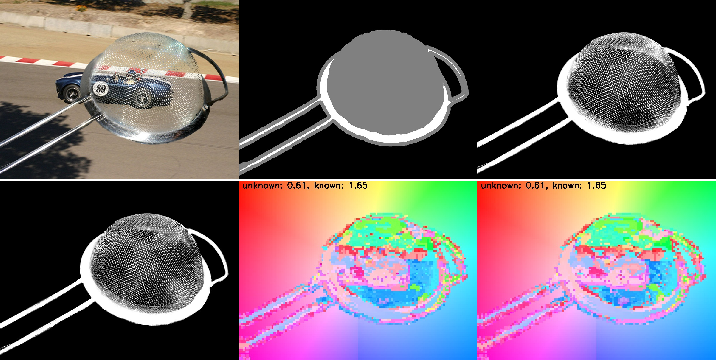
\includegraphics[width = 0.85\columnwidth]{chap5/10261offset.pdf}
	\bicaption{引导上下文注意力图的可视化。第一行从左至右分别为输入图像、trimap图和真实标注;第二行为alpha遮罩估计值、编码器中GCA模块的注意力偏移图和解码器中GCA模块的注意力偏移图}{The visualization of the guided contextual attention map. Top row from left to right, the image, trimap and ground-truth. Second row, the alpha matte prediction, attention offset map from first GCA block in the encoder, offset from GCA block in the decoder}
	\label{fig5:offset}
\end{figure}


\begin{figure}[t]
	\centering
	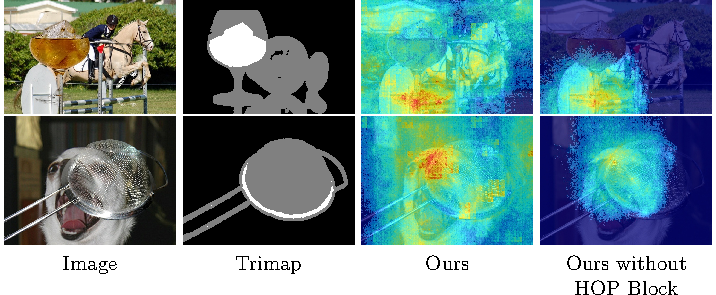
\includegraphics[width = 0.95\columnwidth]{chap5/vis.pdf}
	\bicaption{HOP结构注意力在输入图像上的可视化}{The visualization of attention in our HOP structure on input images}
	\label{fig5:vis}
\end{figure}


\section{本章小结}
在本章中,我们提出了两种基于相似性学习的端到端深度图像抠图方法。所提出的引导上下文注意力抠图方法,以全卷积的方式实现了传统基于相似性的抠图算法中的信息传播过程。其中的引导上下文注意力模块通过借助图像外观信息的引导,实现alpha特征之间的不透明度传播。而所提出的层次化不透明度传播抠图方法,则利用全局和局部模块以实现不同语义级别上的层次化信息传播。
所提出的两种方法,都通过数据驱动的训练,以网络模型的形式学习图像像素间相似性的计算方式。并依据网络模型计算出的相似性,实现不透明度信息的传播。
大量的定量实验和消融实验证明了本章所提出的抠图方法及其中的模块、数据增广方式的有效性和优越性。